% Activate the following line by filling in the right side. If for example the name of the root file is Main.tex, write
% "...root = Main.tex" if the chapter file is in the same directory, and "...root = ../Main.tex" if the chapter is in a subdirectory.
 
%!TEX root =  ../Thesis.tex

\chapter[Signal Kinematics]{Signal Kinematics}

 
\section{Signal Jet Kinematics}

Once the trigger and cuts have been applied to the data, the events that remain can be signal, background, or a mixture of the two.  
It then falls to understanding the kinematics of the signal and background to look for features that can
provide enough discrimination to detect the presence of the signal.  In this case, that means reconstructing
the invariant mass of the leading 2 jets in the event, which will create a smoothly falling power
law distribution in QCD background but a resonance structure in signal.  The kinematics of the signal
distribution then come into play in a few major ways
\begin{itemize}
    \item Signal Jet \pt Distributions:  By examining the \pt distributions of the Higgs daughters, and the associated $b$-jet(s), we can get a better understanding of what might be optimal jet \pt cuts for future iterationsof this analysis 
    \item Signal Jet Combinatorics: A perfectly good signal event can be inadvertently turned into a type of background if the associated $b$-jet is chosen when reconstructing the Higgs; unfortunately these combinatorial mistakes can arise easily when there are 3 $b$-jets but only two jets being used for reconstruction
    \item Mass Resolution: The Higgs resonance width is $m_A$/tan$\beta$ dependent, with inherent widths
up to a few tens of GeV; however, if energy is lost to FSR, the resonance can be much wider and this makes
the signal much more difficult to distinguish from the background
\end{itemize}


\section{Signal Jet \pt Distributions}

An important place to start is with the \pt distributions of the jets after the trigger
and cuts have been applied.  Using truth-matching in the Monte Carlo, we can identify
which jets are daughters of the Higgs and which are associated $b$-jet(s).  Since
the Higgs is a heavy particle, its decay jets tend to have higher \pt than the associated
$b$-jet(s), which can be seen in Figure~\ref{fig:pt_higgs_and_associated_jets}. 
However, in this plot, there has been $b$-tagging applied so an important potential
component is missing: how does the event topology change when we also include 
non-$b$-jets, which can potentially be high \pt as well.   

%----------------------------------------------
\begin{figure}[H]
    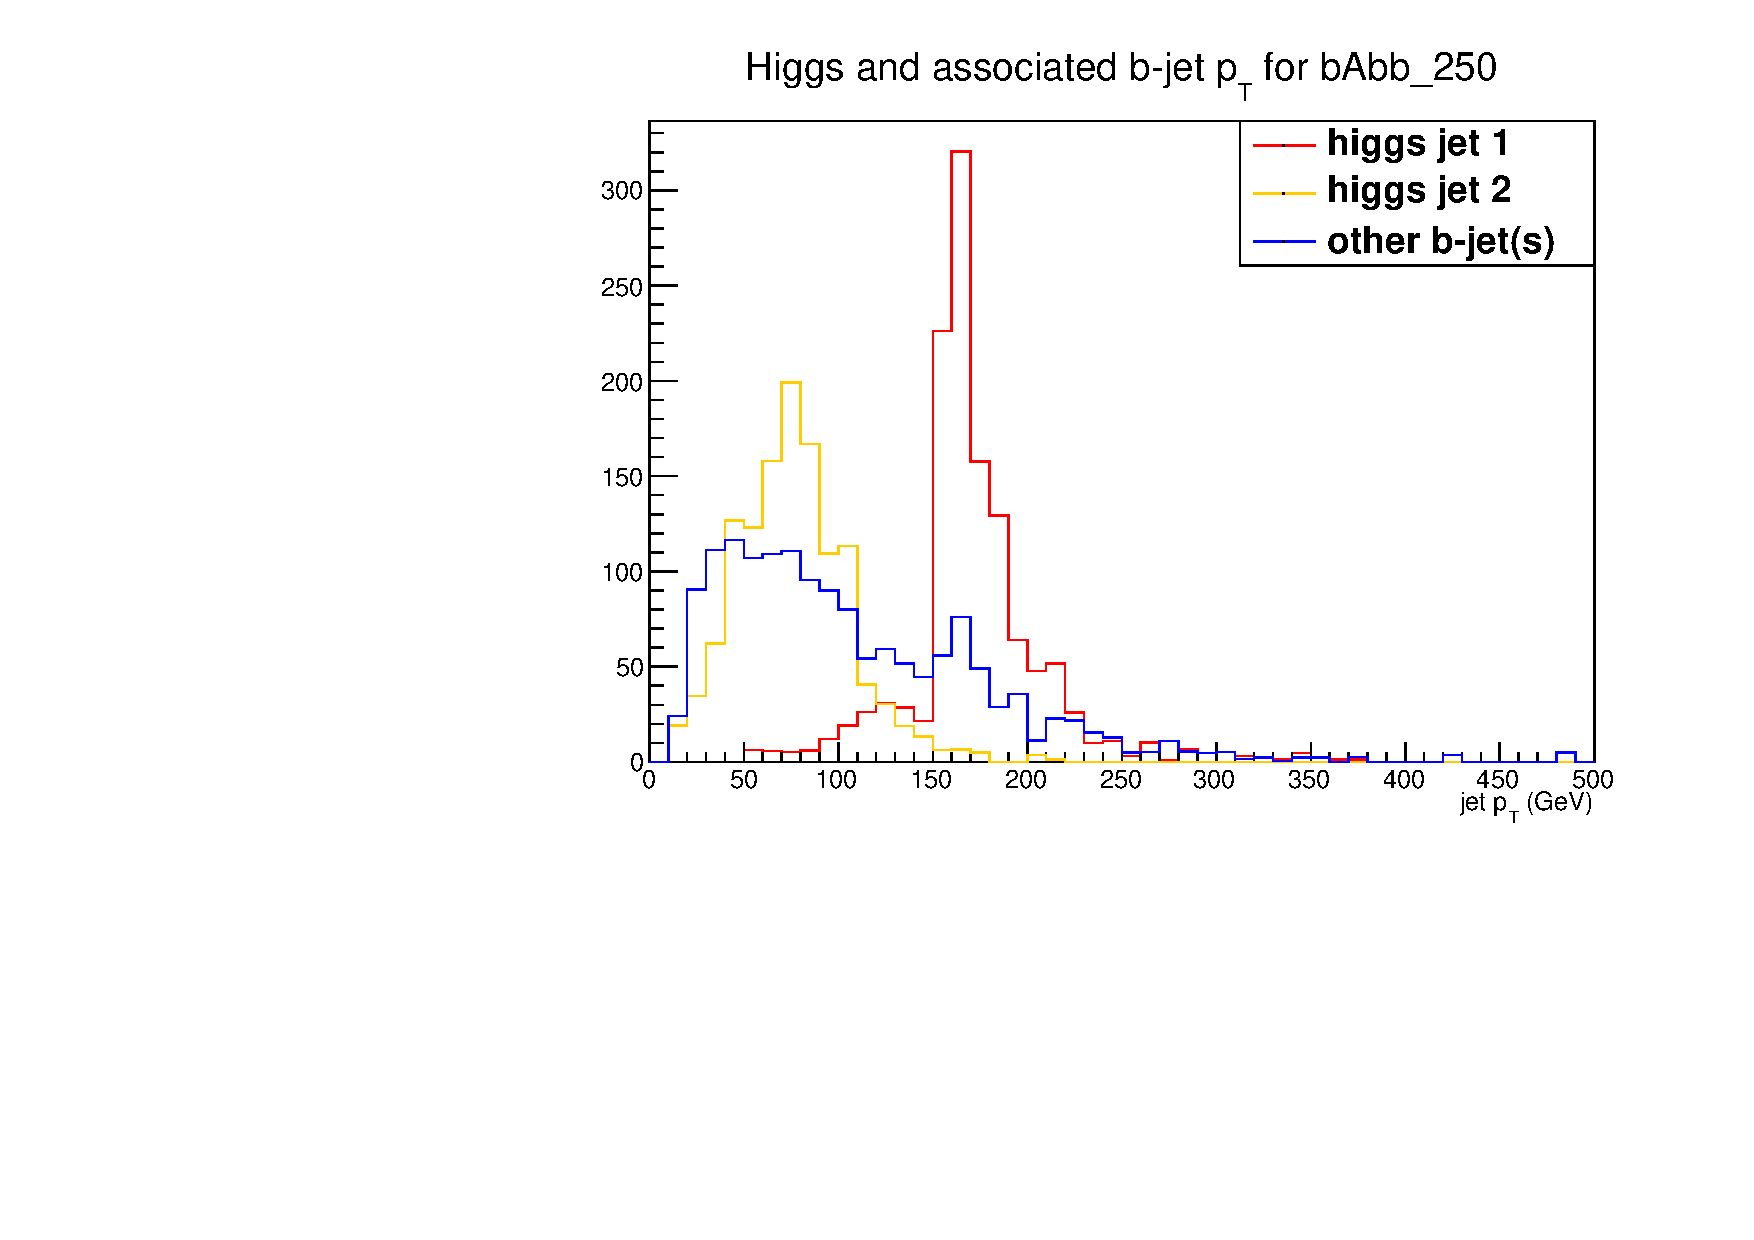
\includegraphics[width=0.3\textwidth]{SignalKin/jet_pt_compare_bAbb_250.pdf}
    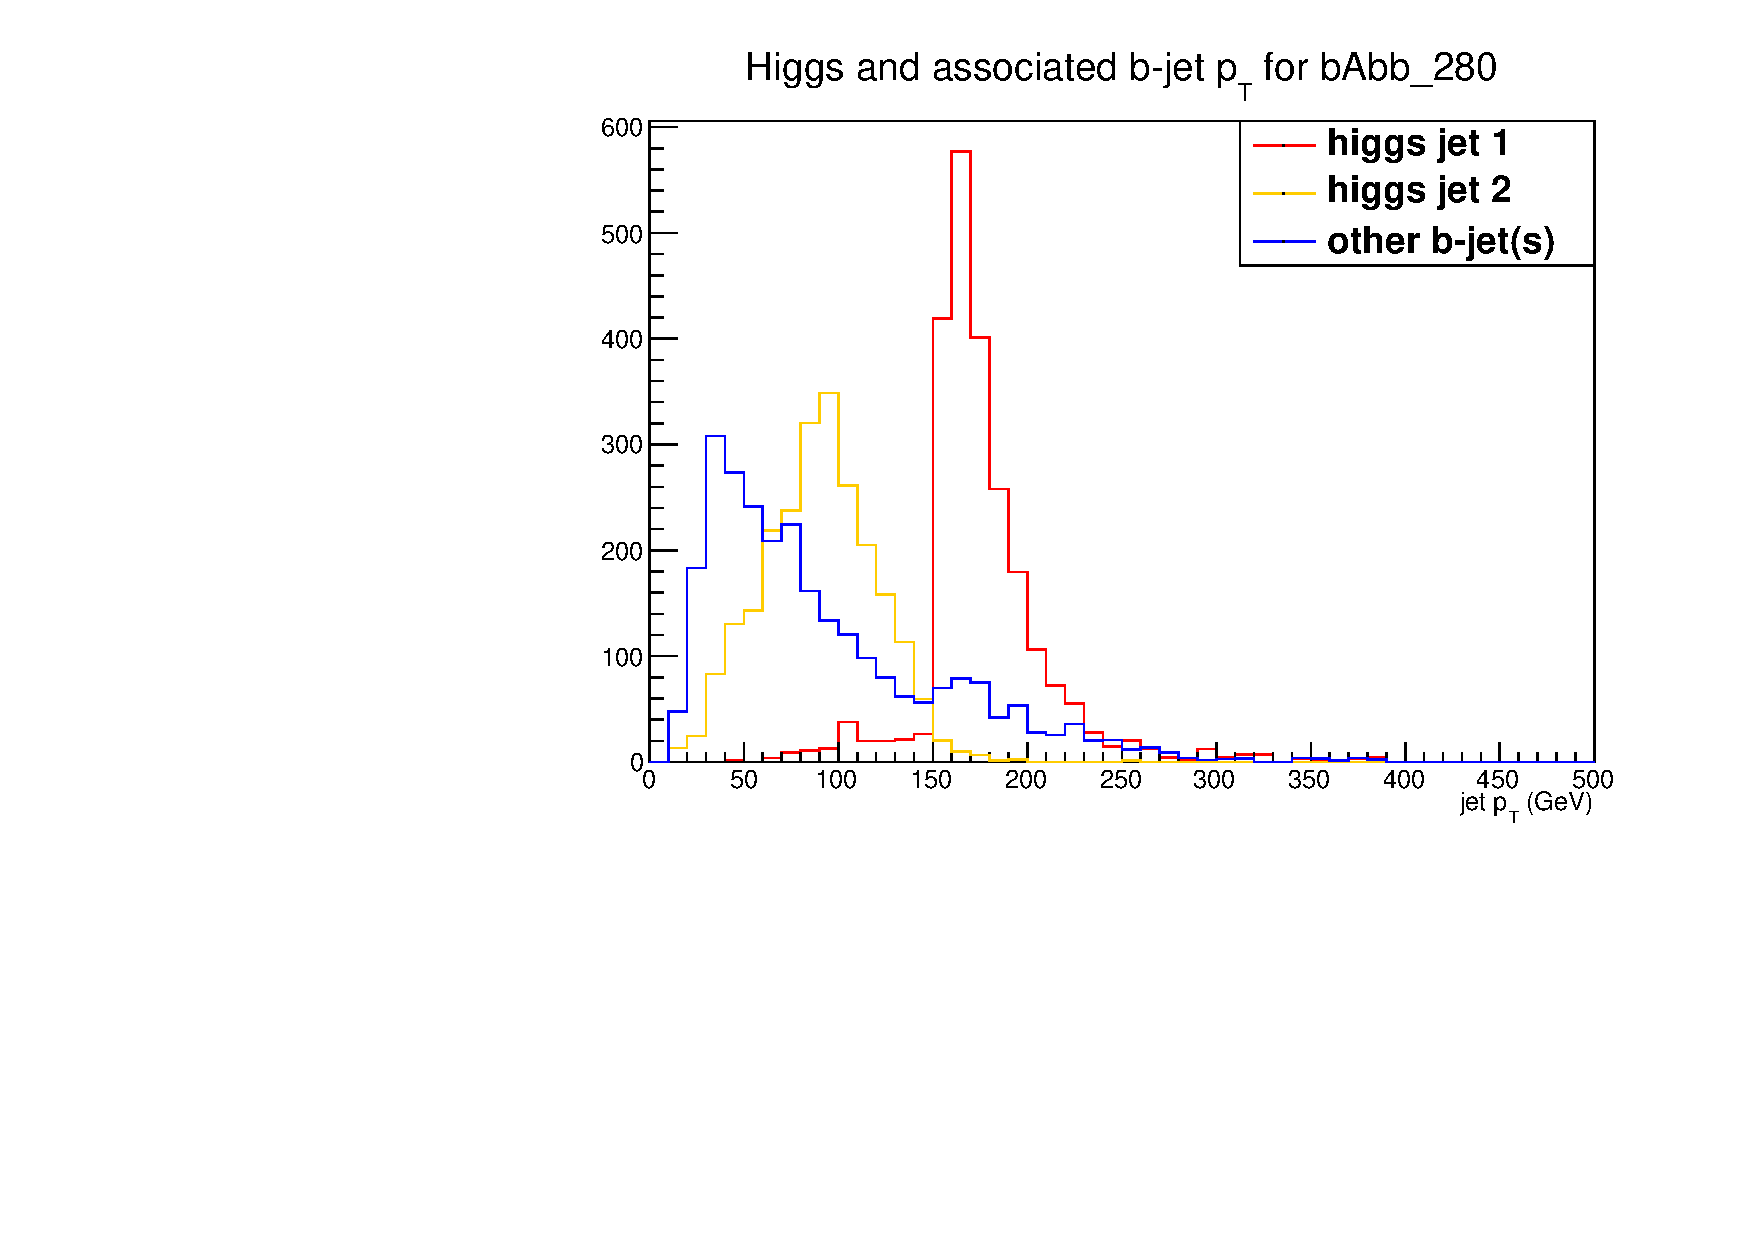
\includegraphics[width=0.3\textwidth]{SignalKin/jet_pt_compare_bAbb_280.pdf}
    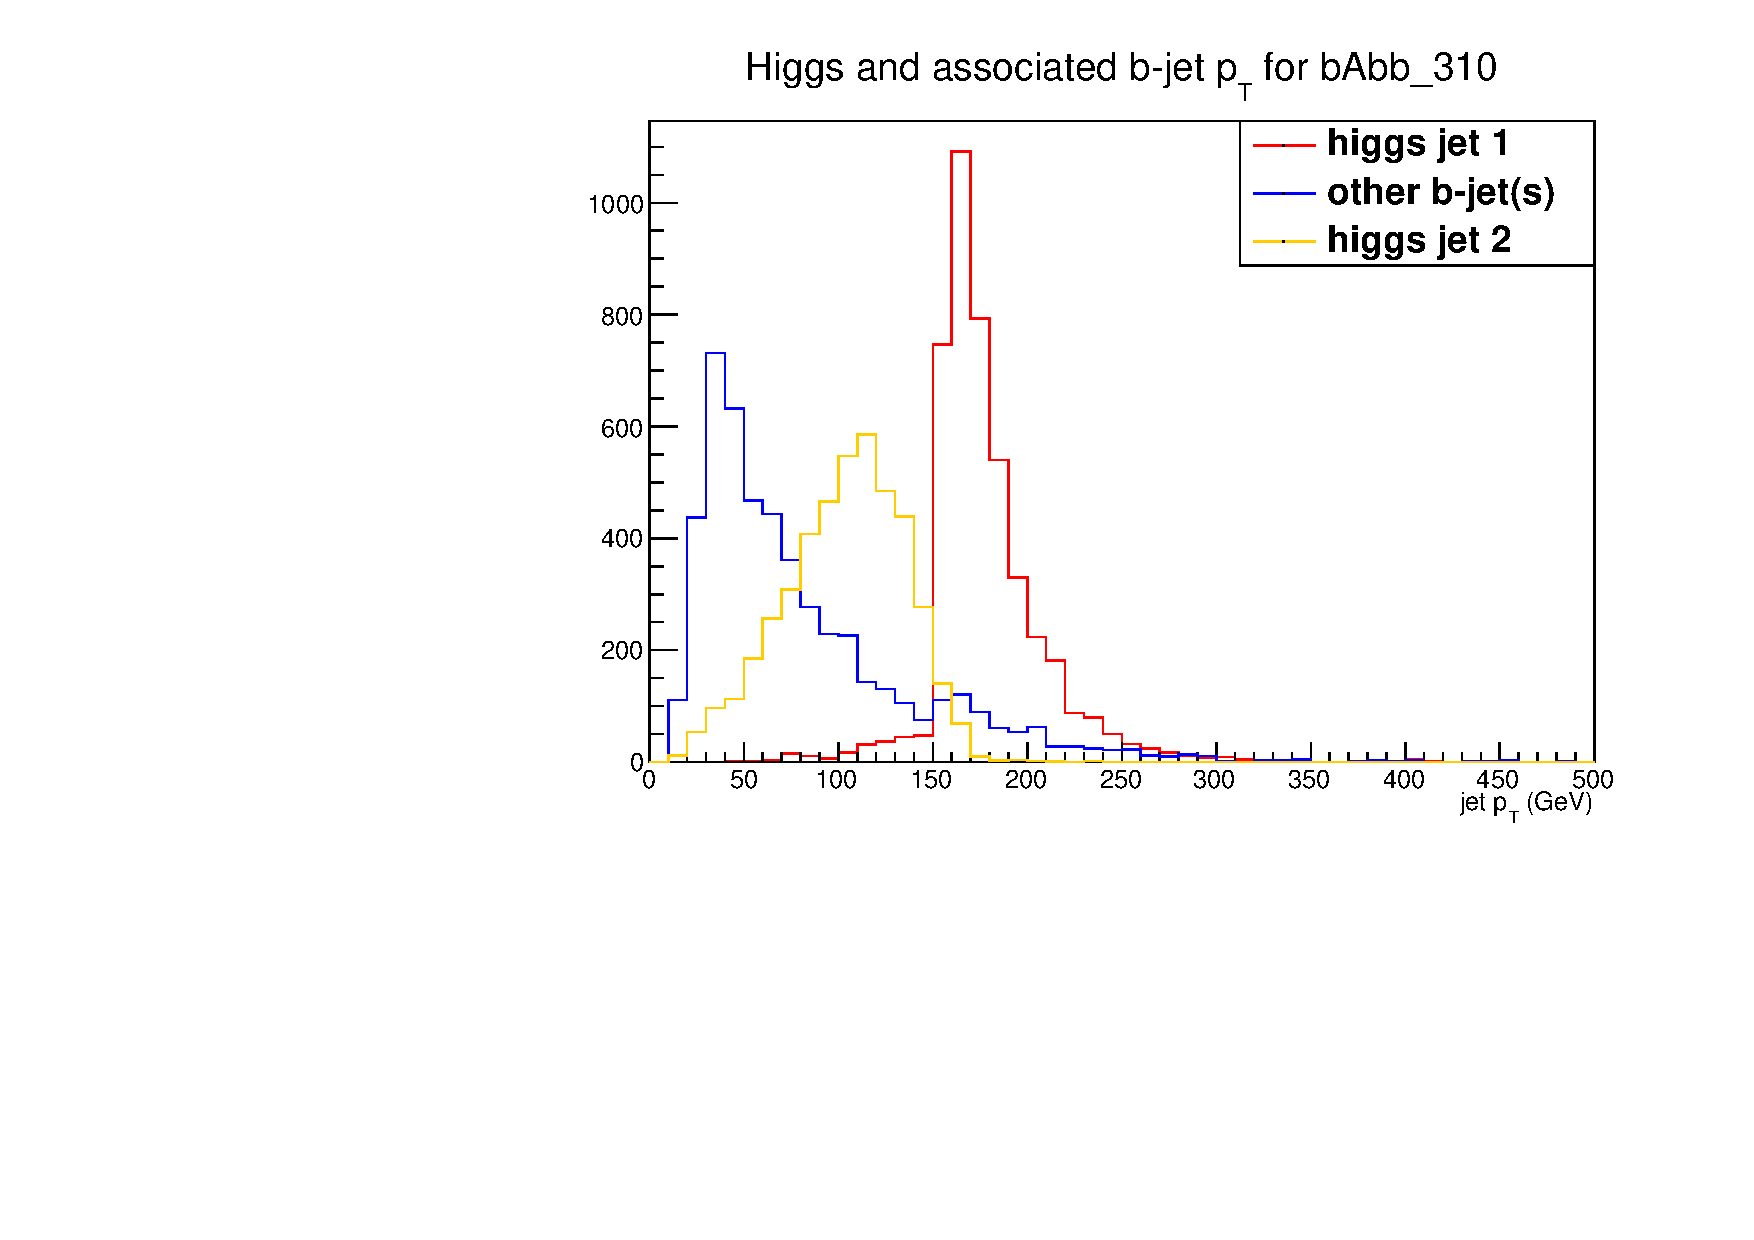
\includegraphics[width=0.3\textwidth]{SignalKin/jet_pt_compare_bAbb_310.pdf}
    \newline
    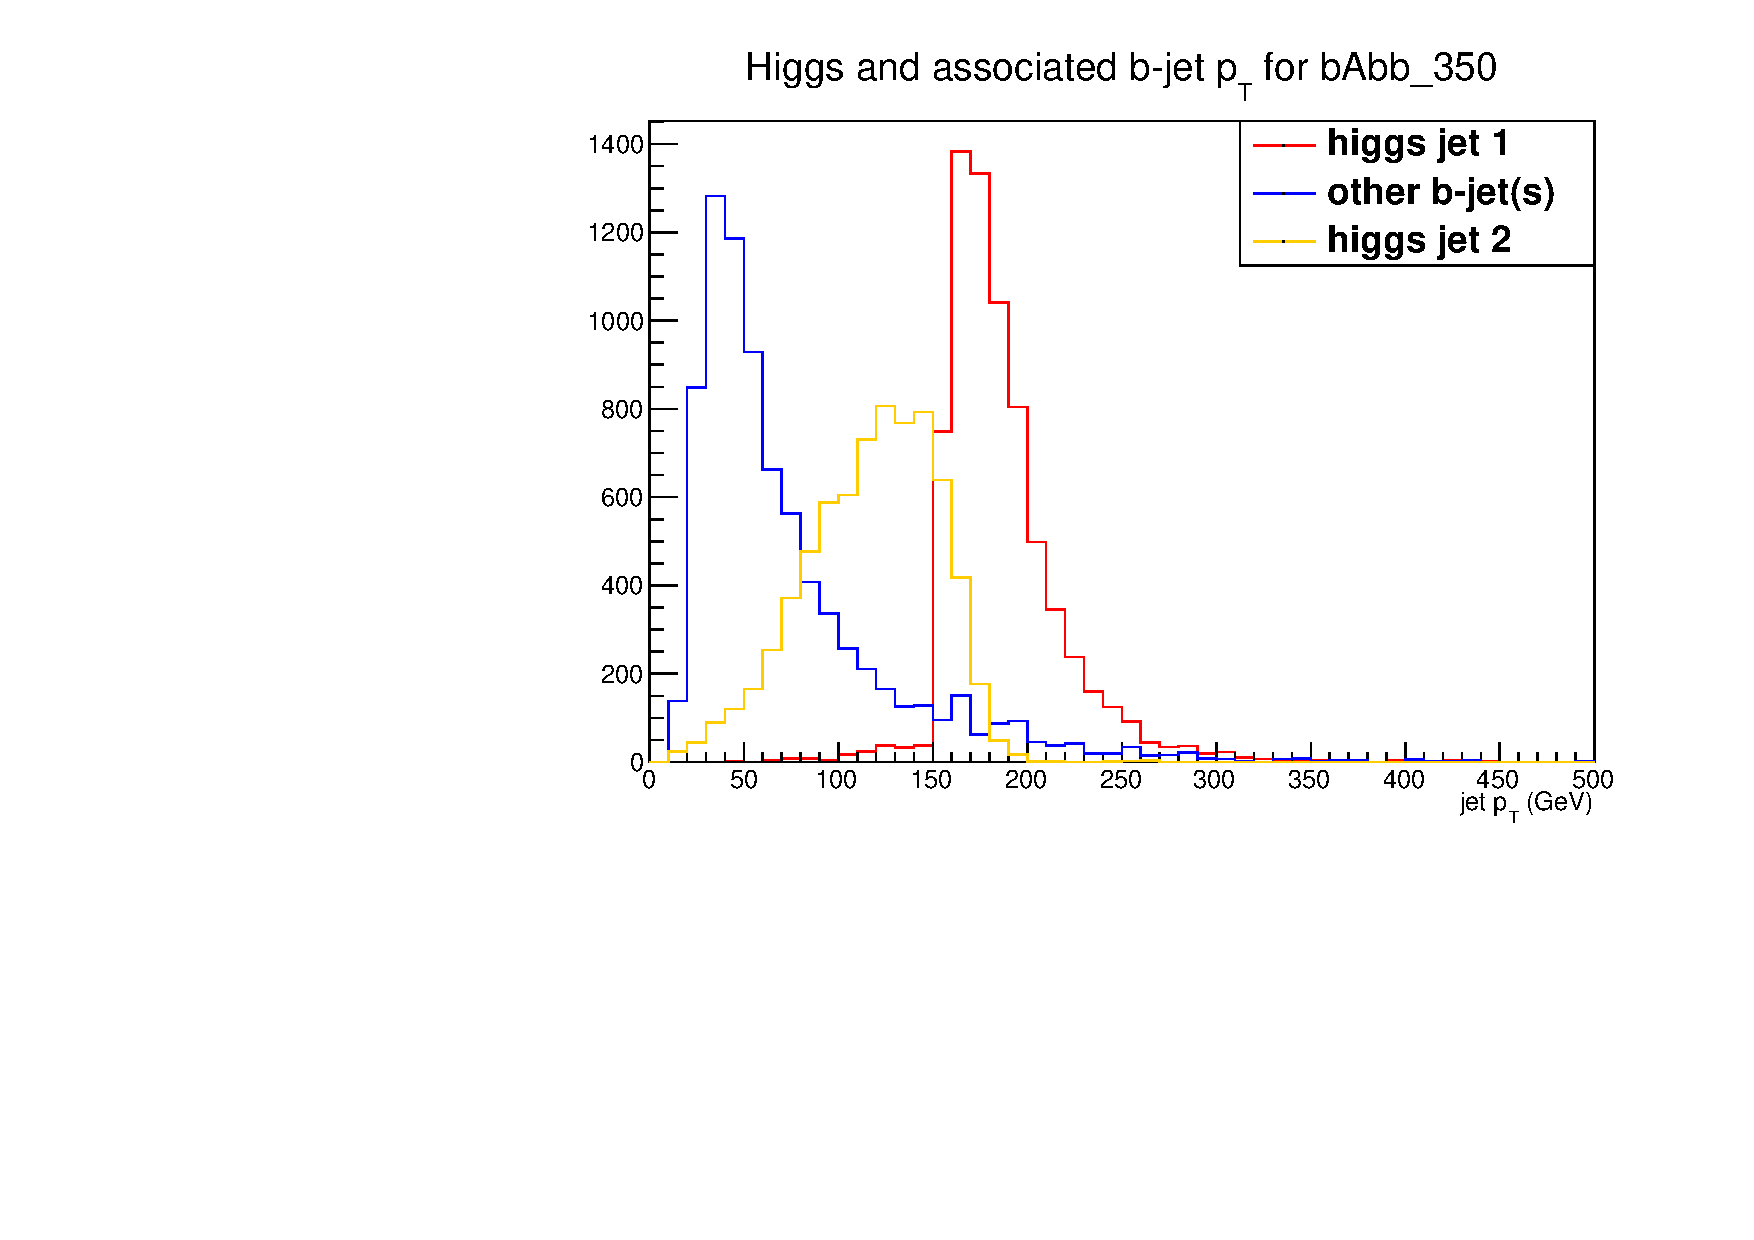
\includegraphics[width=0.3\textwidth]{SignalKin/jet_pt_compare_bAbb_350.pdf}
    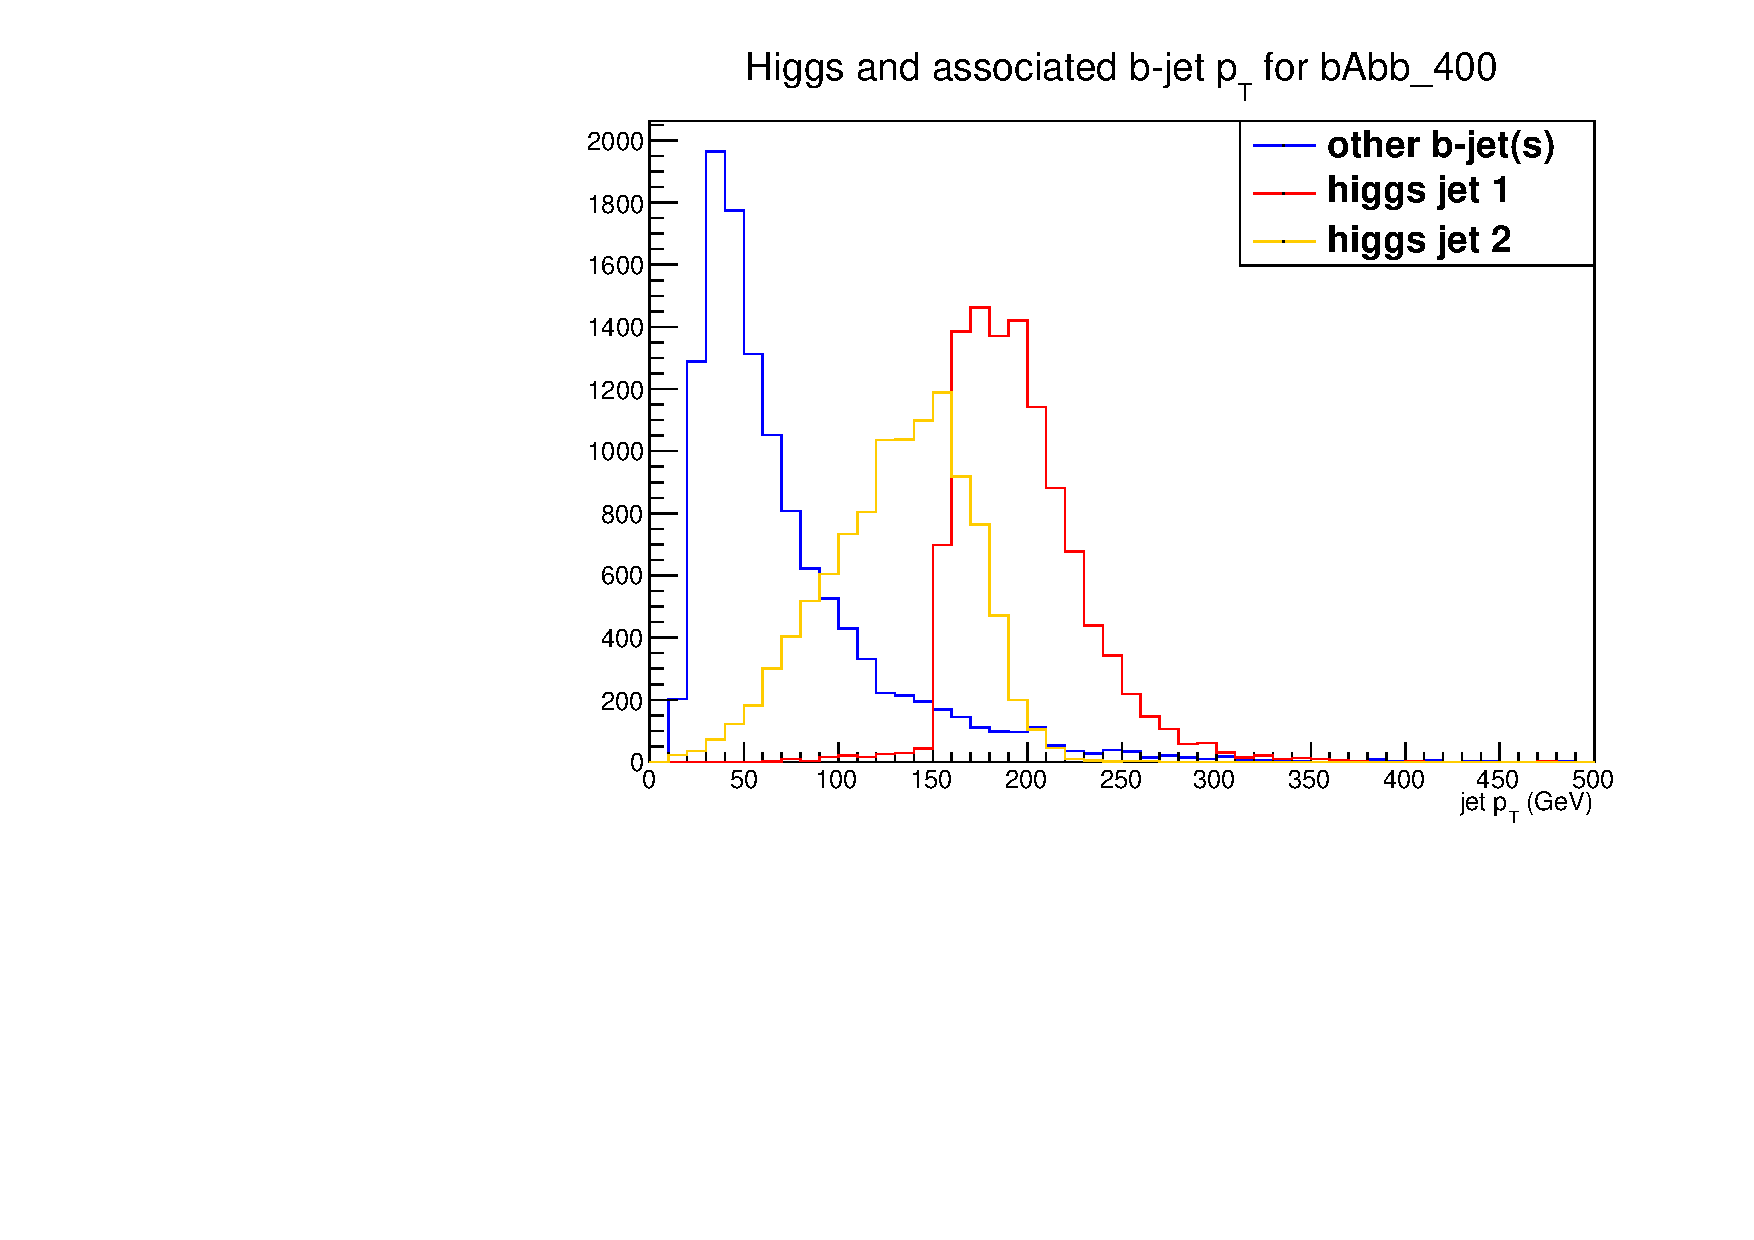
\includegraphics[width=0.3\textwidth]{SignalKin/jet_pt_compare_bAbb_400.pdf}
    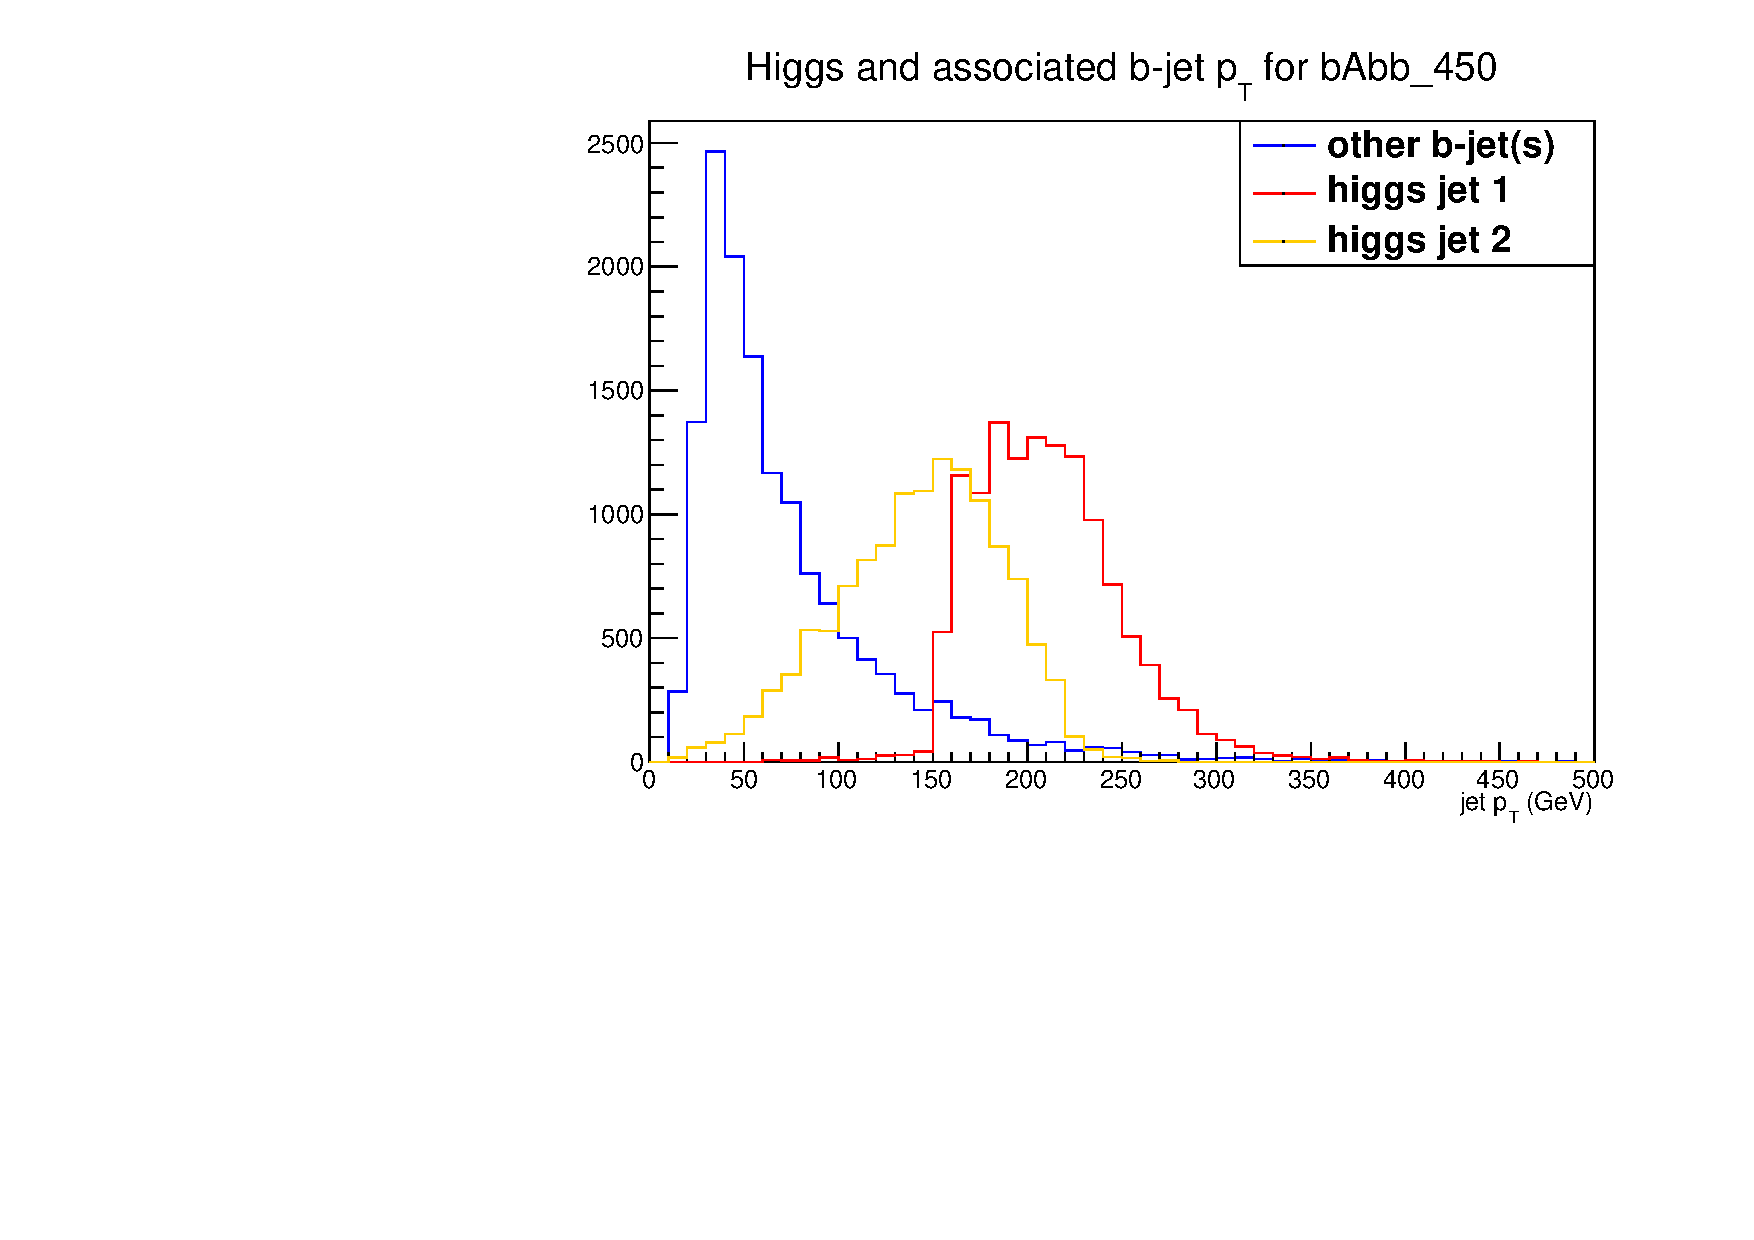
\includegraphics[width=0.3\textwidth]{SignalKin/jet_pt_compare_bAbb_450.pdf}
    \newline
    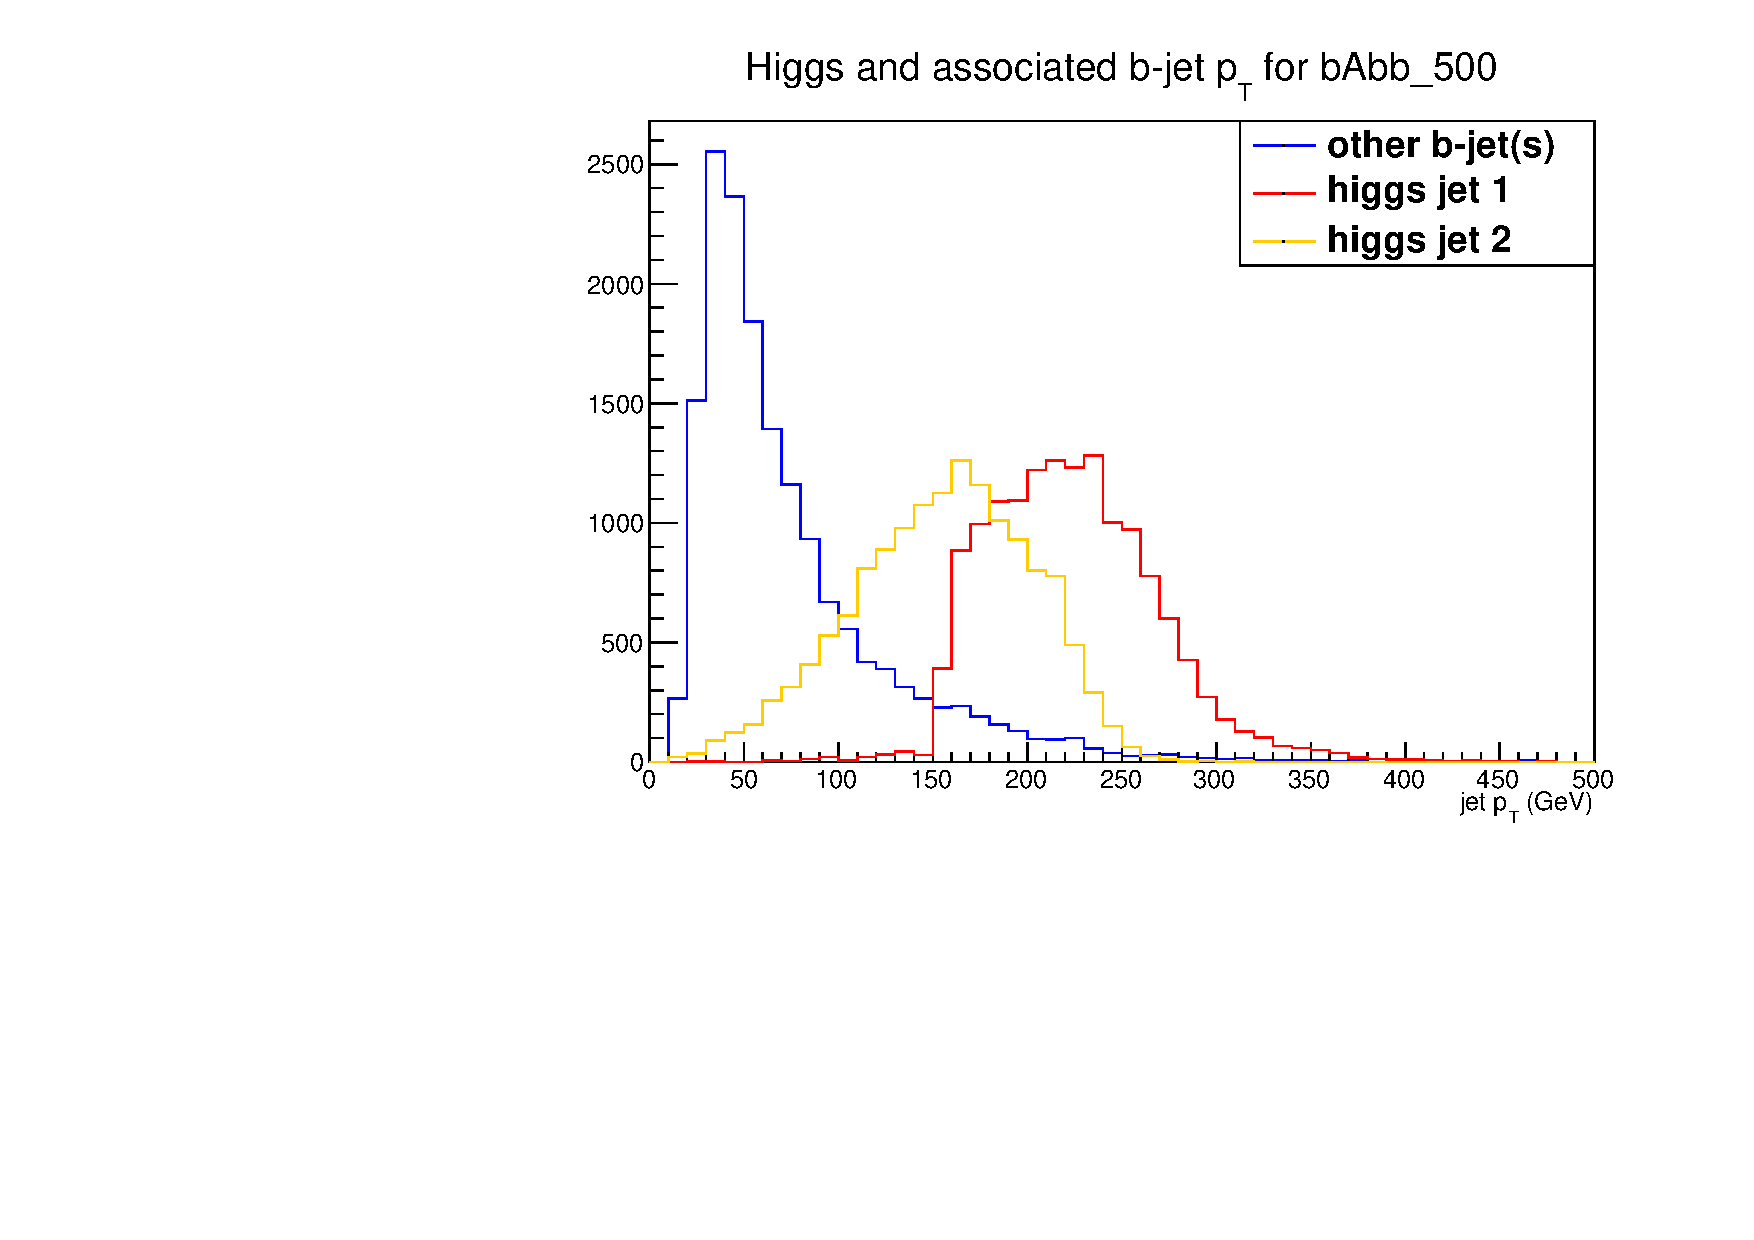
\includegraphics[width=0.3\textwidth]{SignalKin/jet_pt_compare_bAbb_500.pdf}
    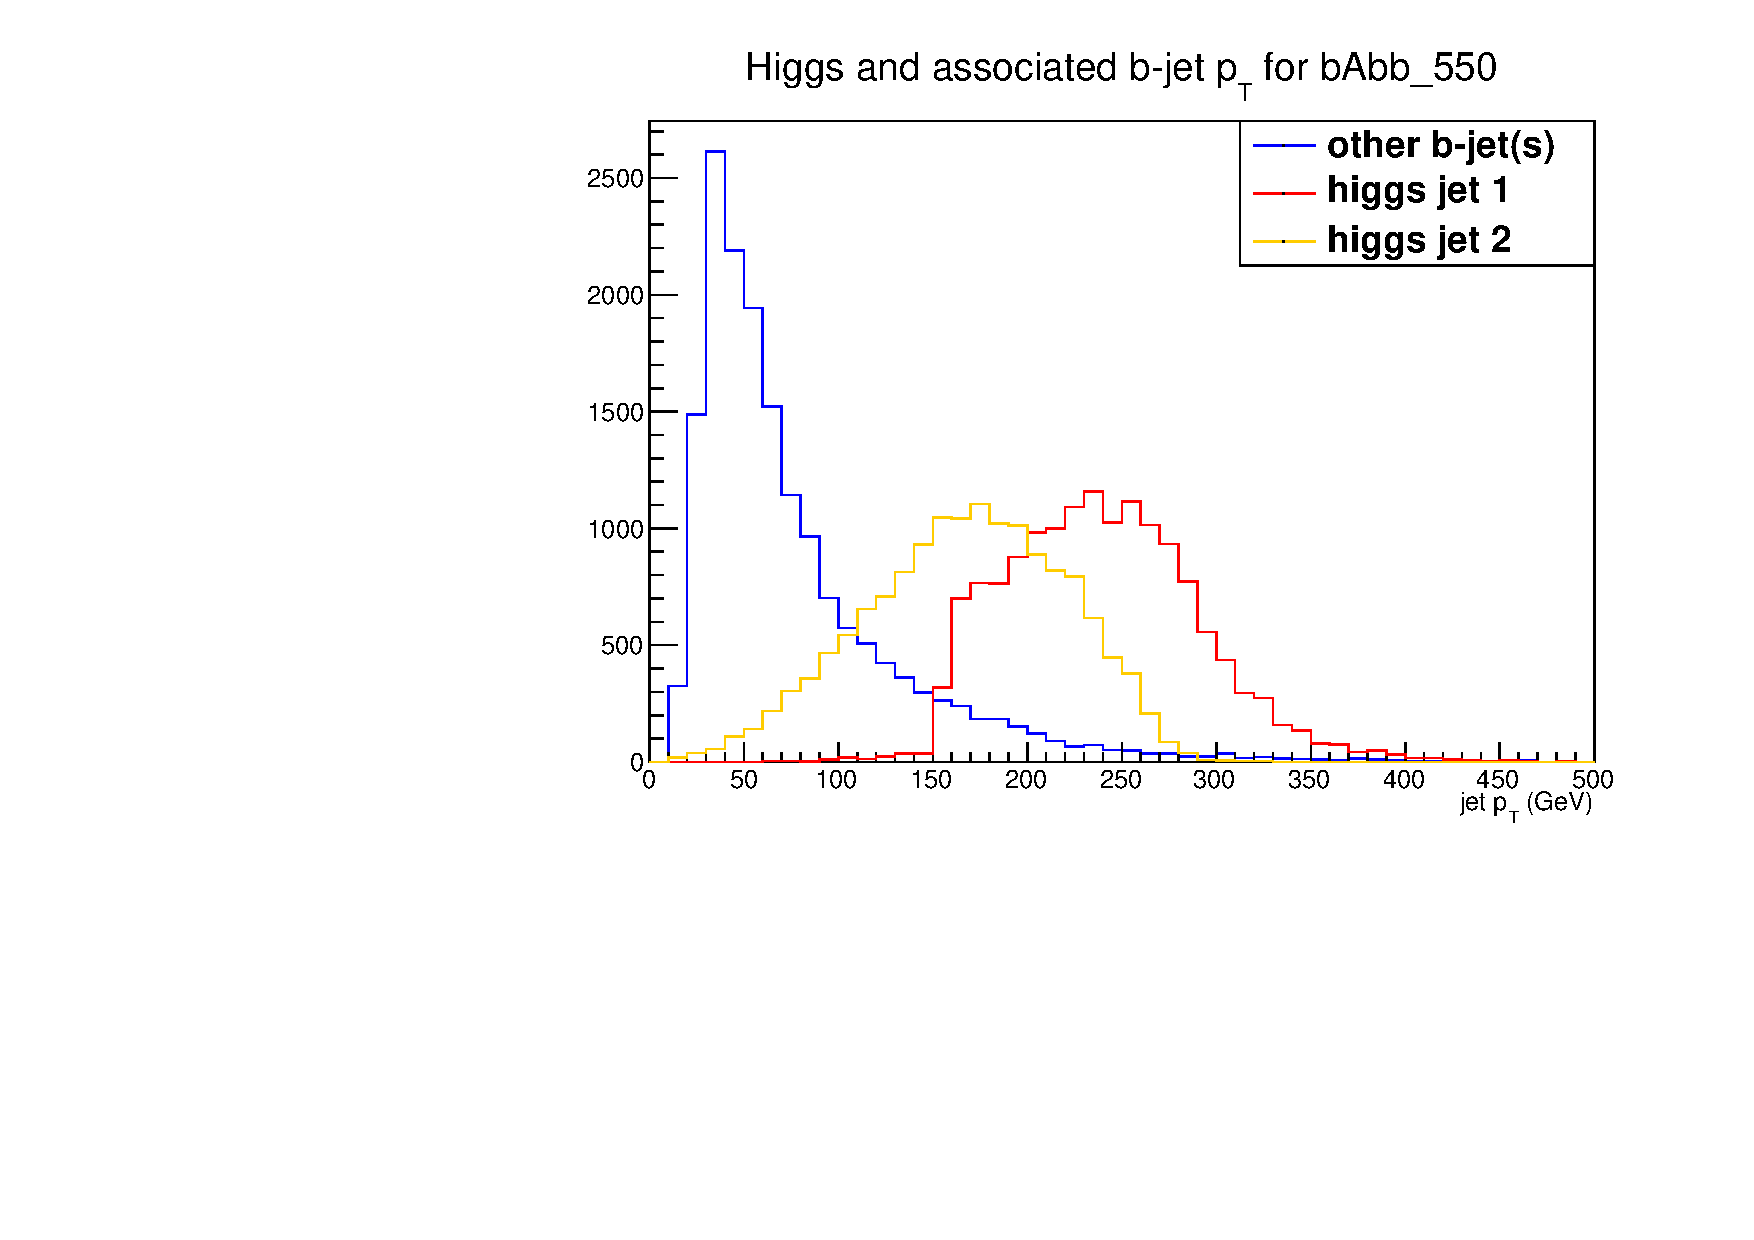
\includegraphics[width=0.3\textwidth]{SignalKin/jet_pt_compare_bAbb_550.pdf}
    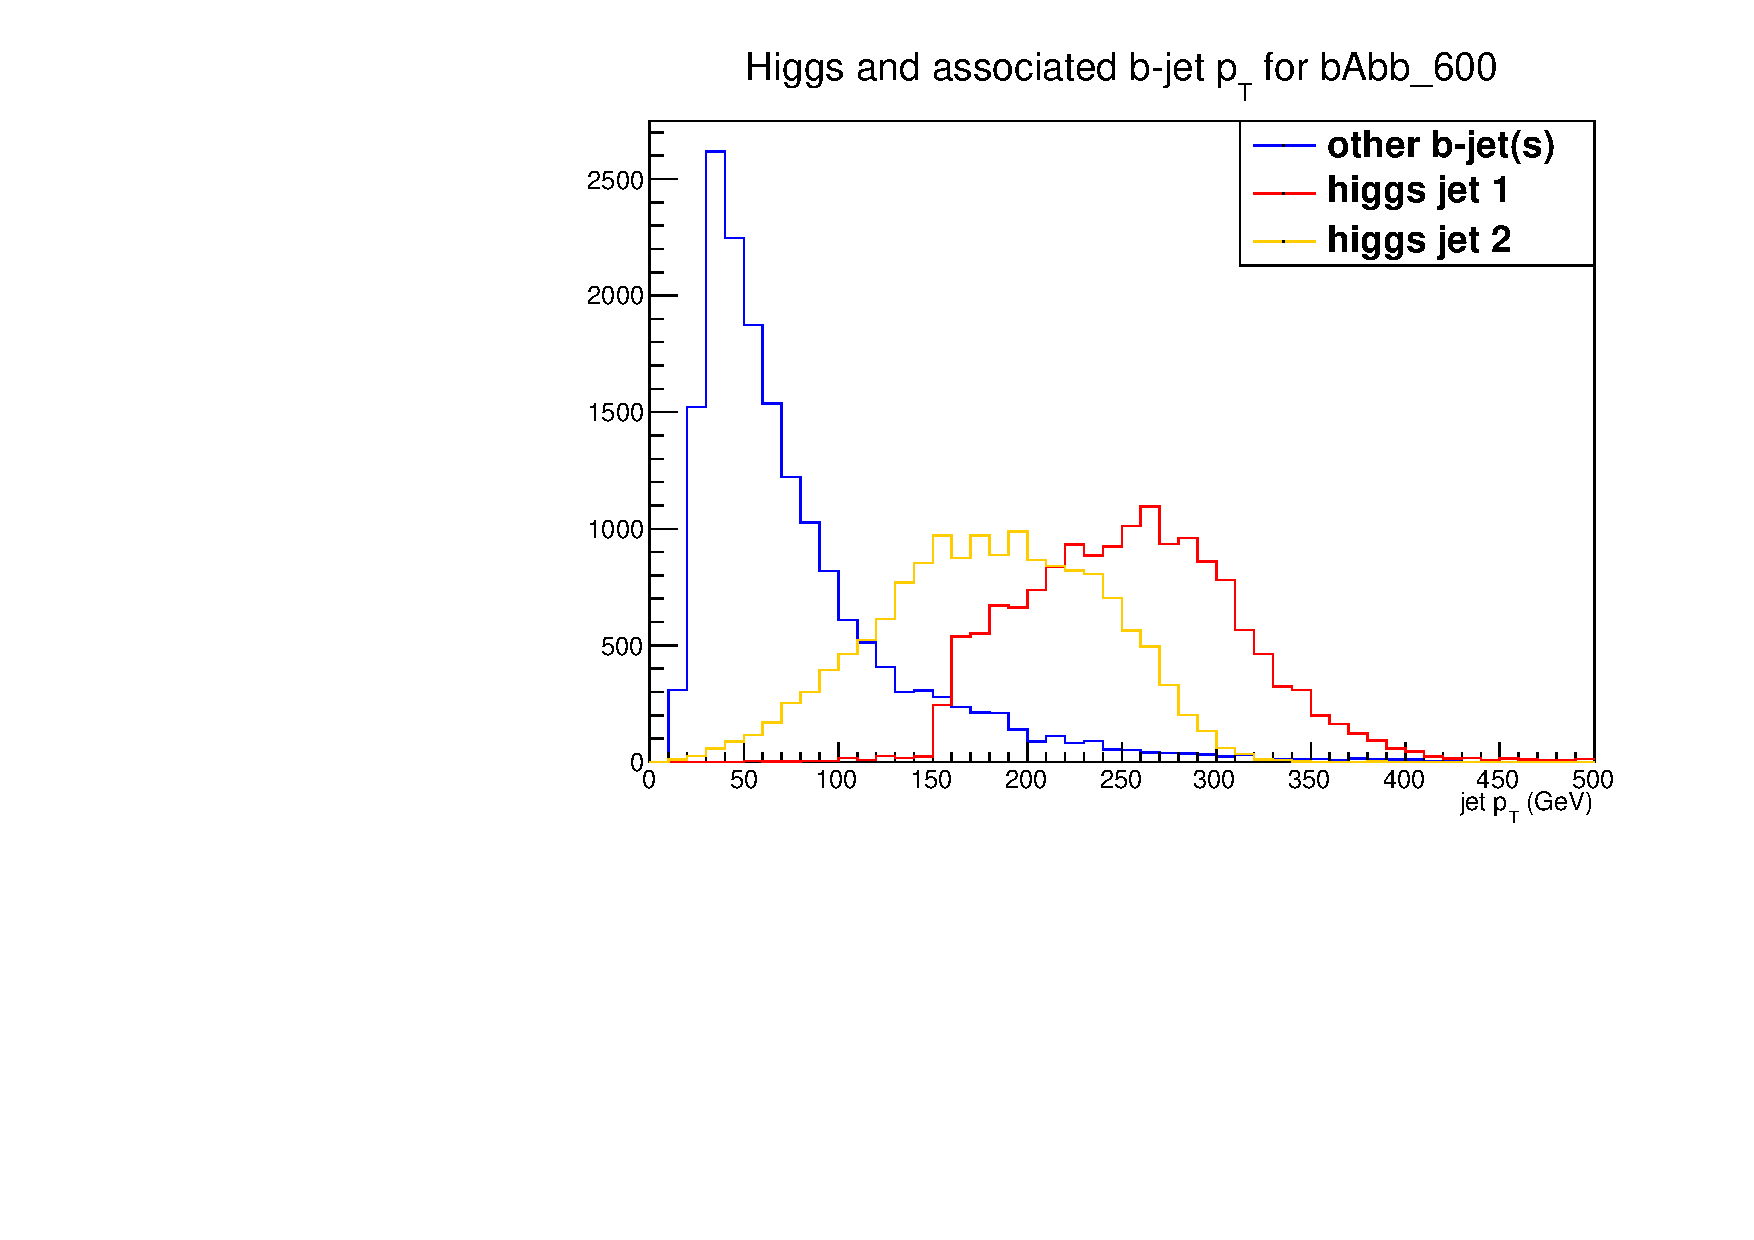
\includegraphics[width=0.3\textwidth]{SignalKin/jet_pt_compare_bAbb_600.pdf}
    \newline
    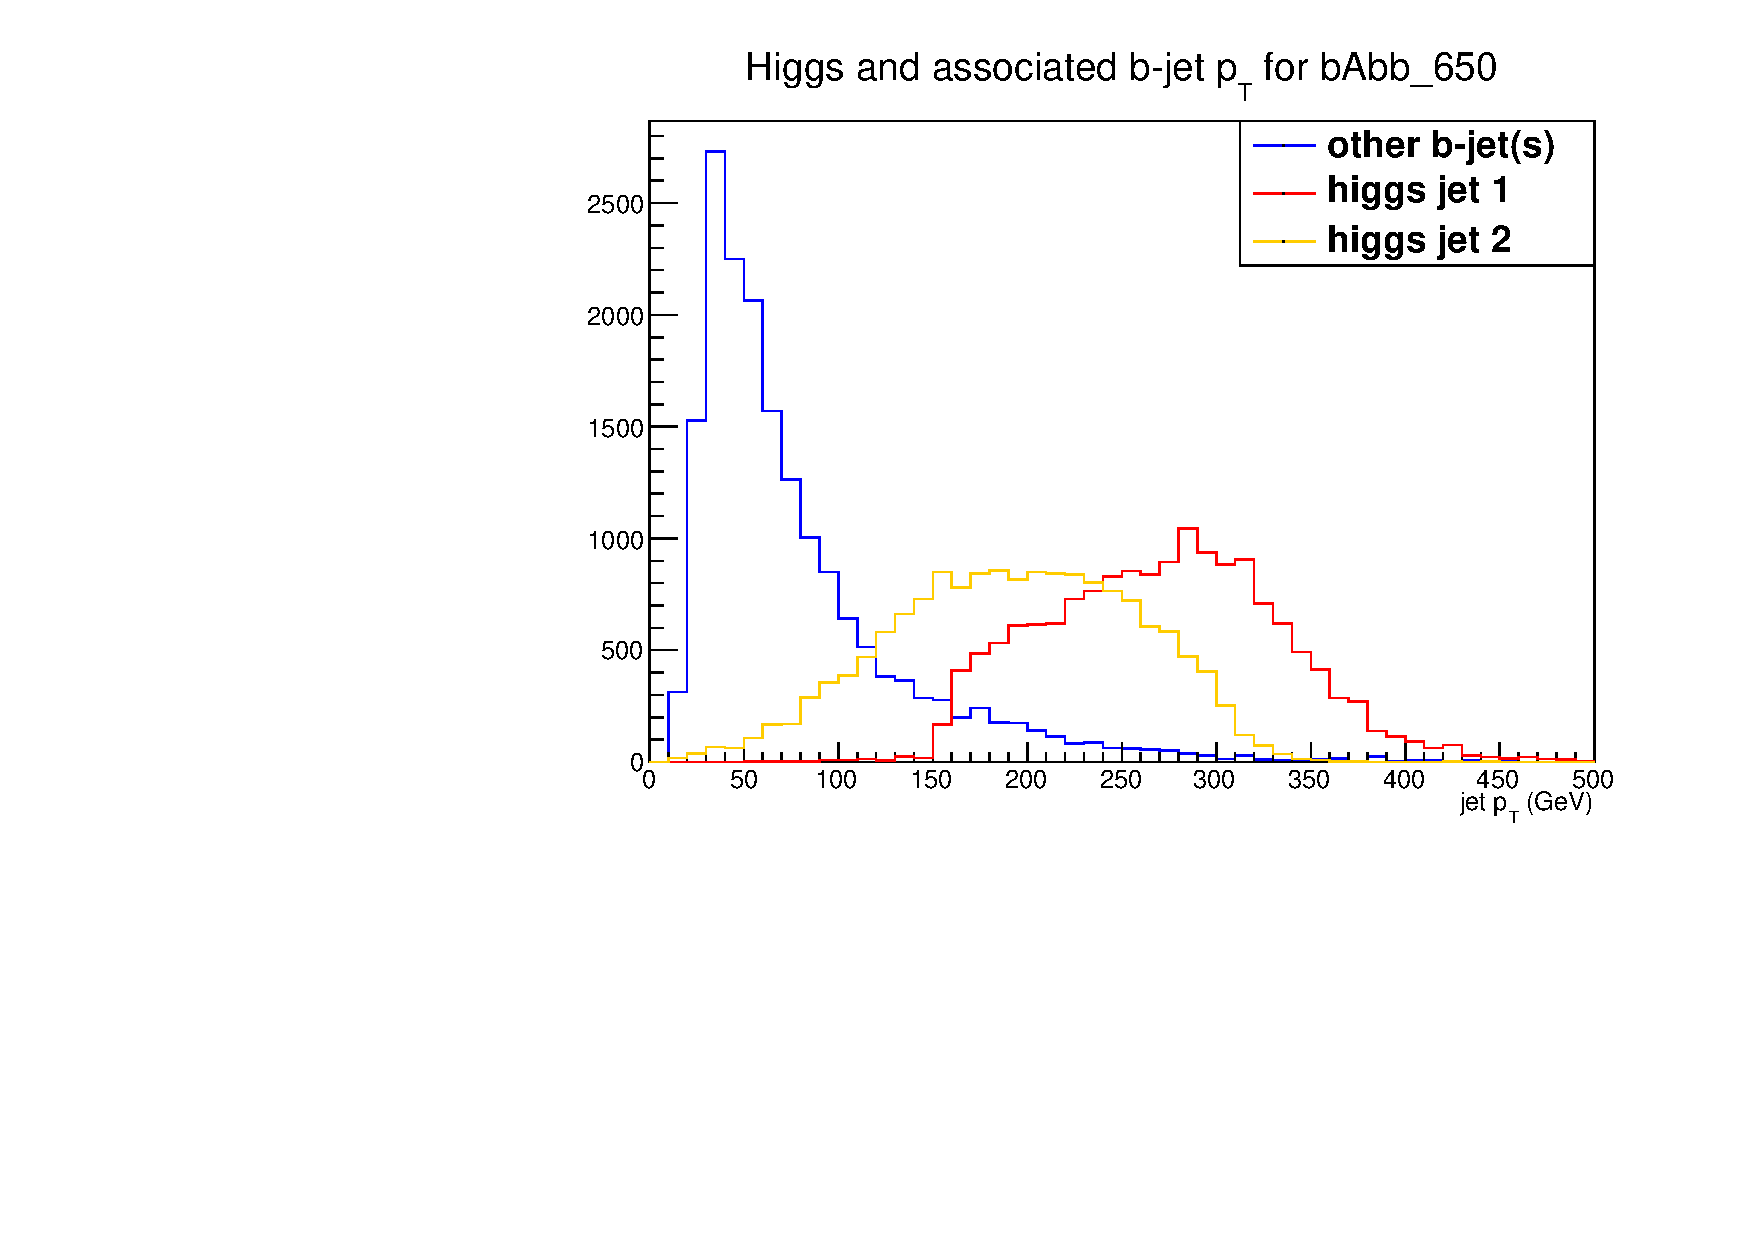
\includegraphics[width=0.3\textwidth]{SignalKin/jet_pt_compare_bAbb_650.pdf}
    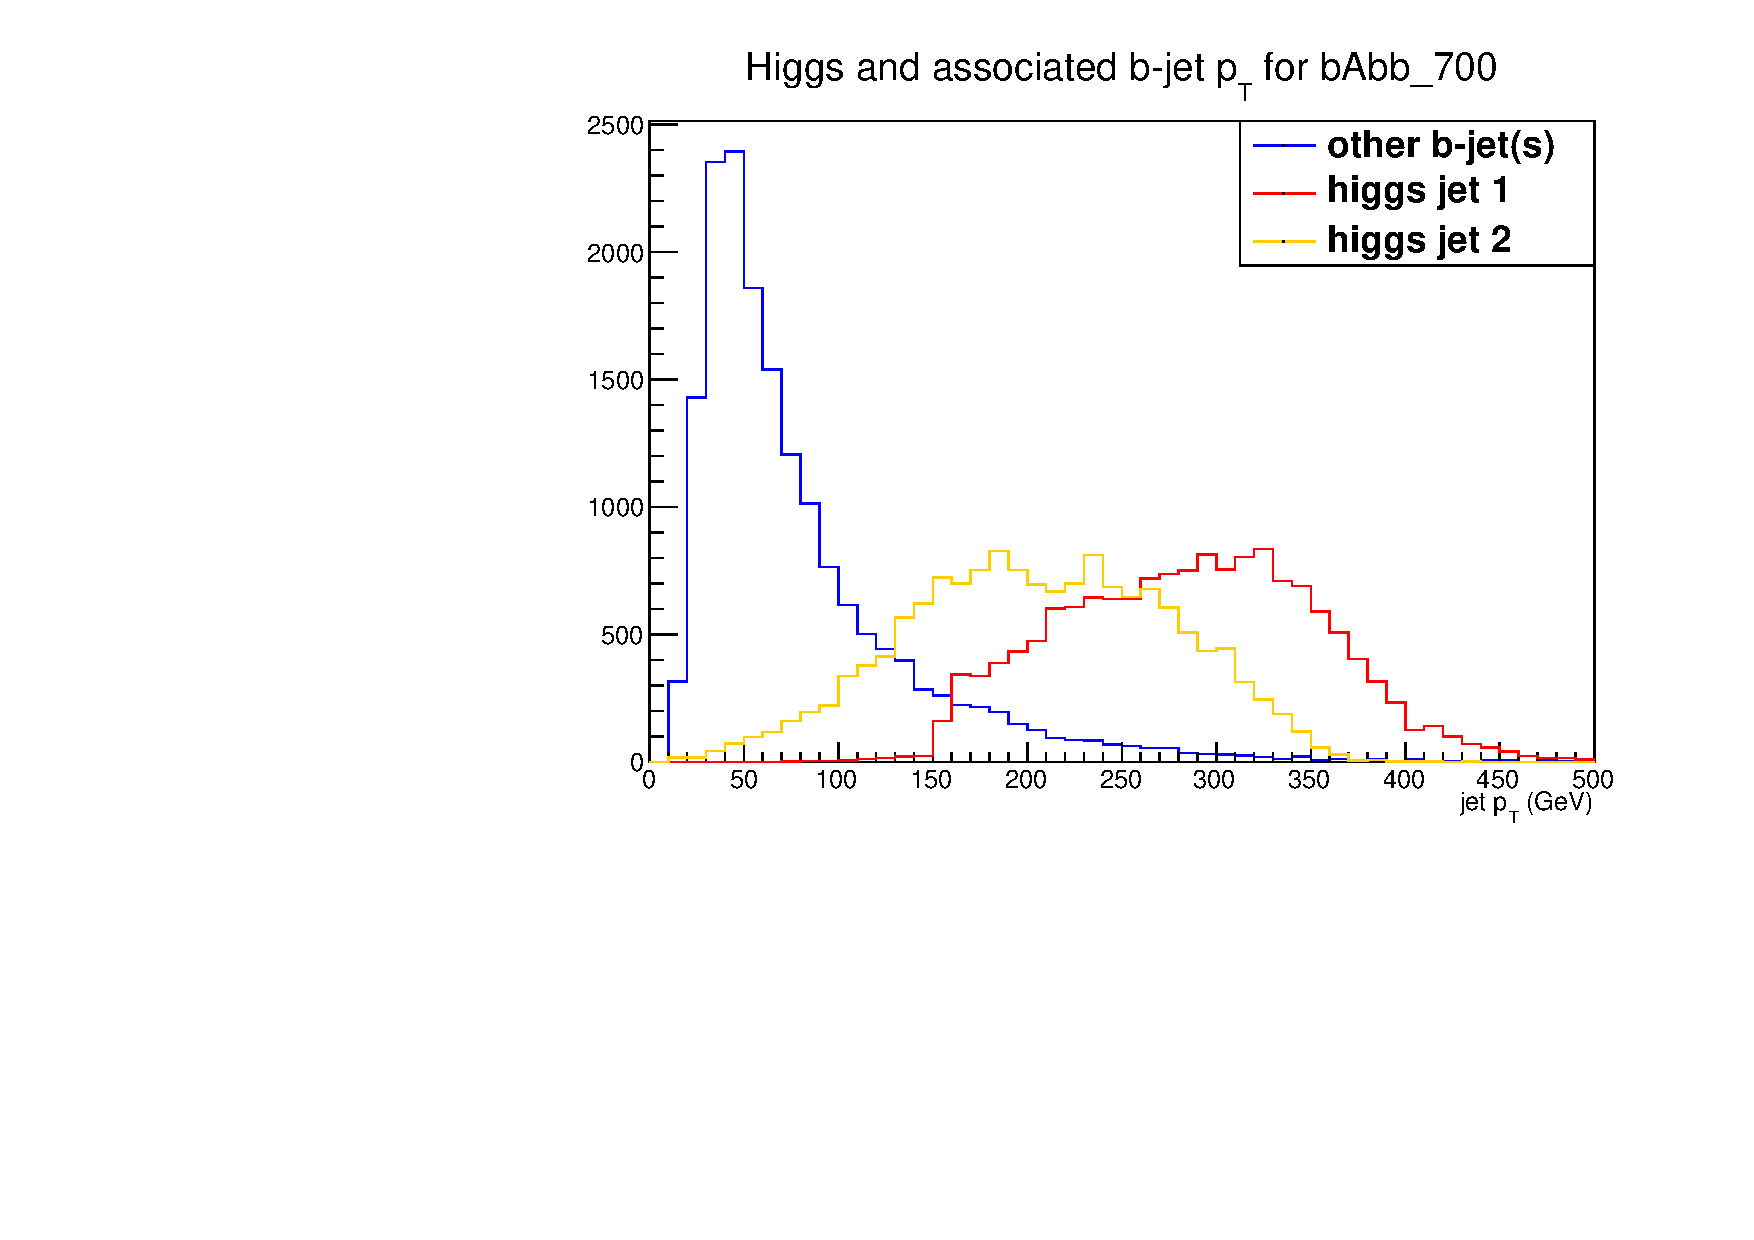
\includegraphics[width=0.3\textwidth]{SignalKin/jet_pt_compare_bAbb_700.pdf}
    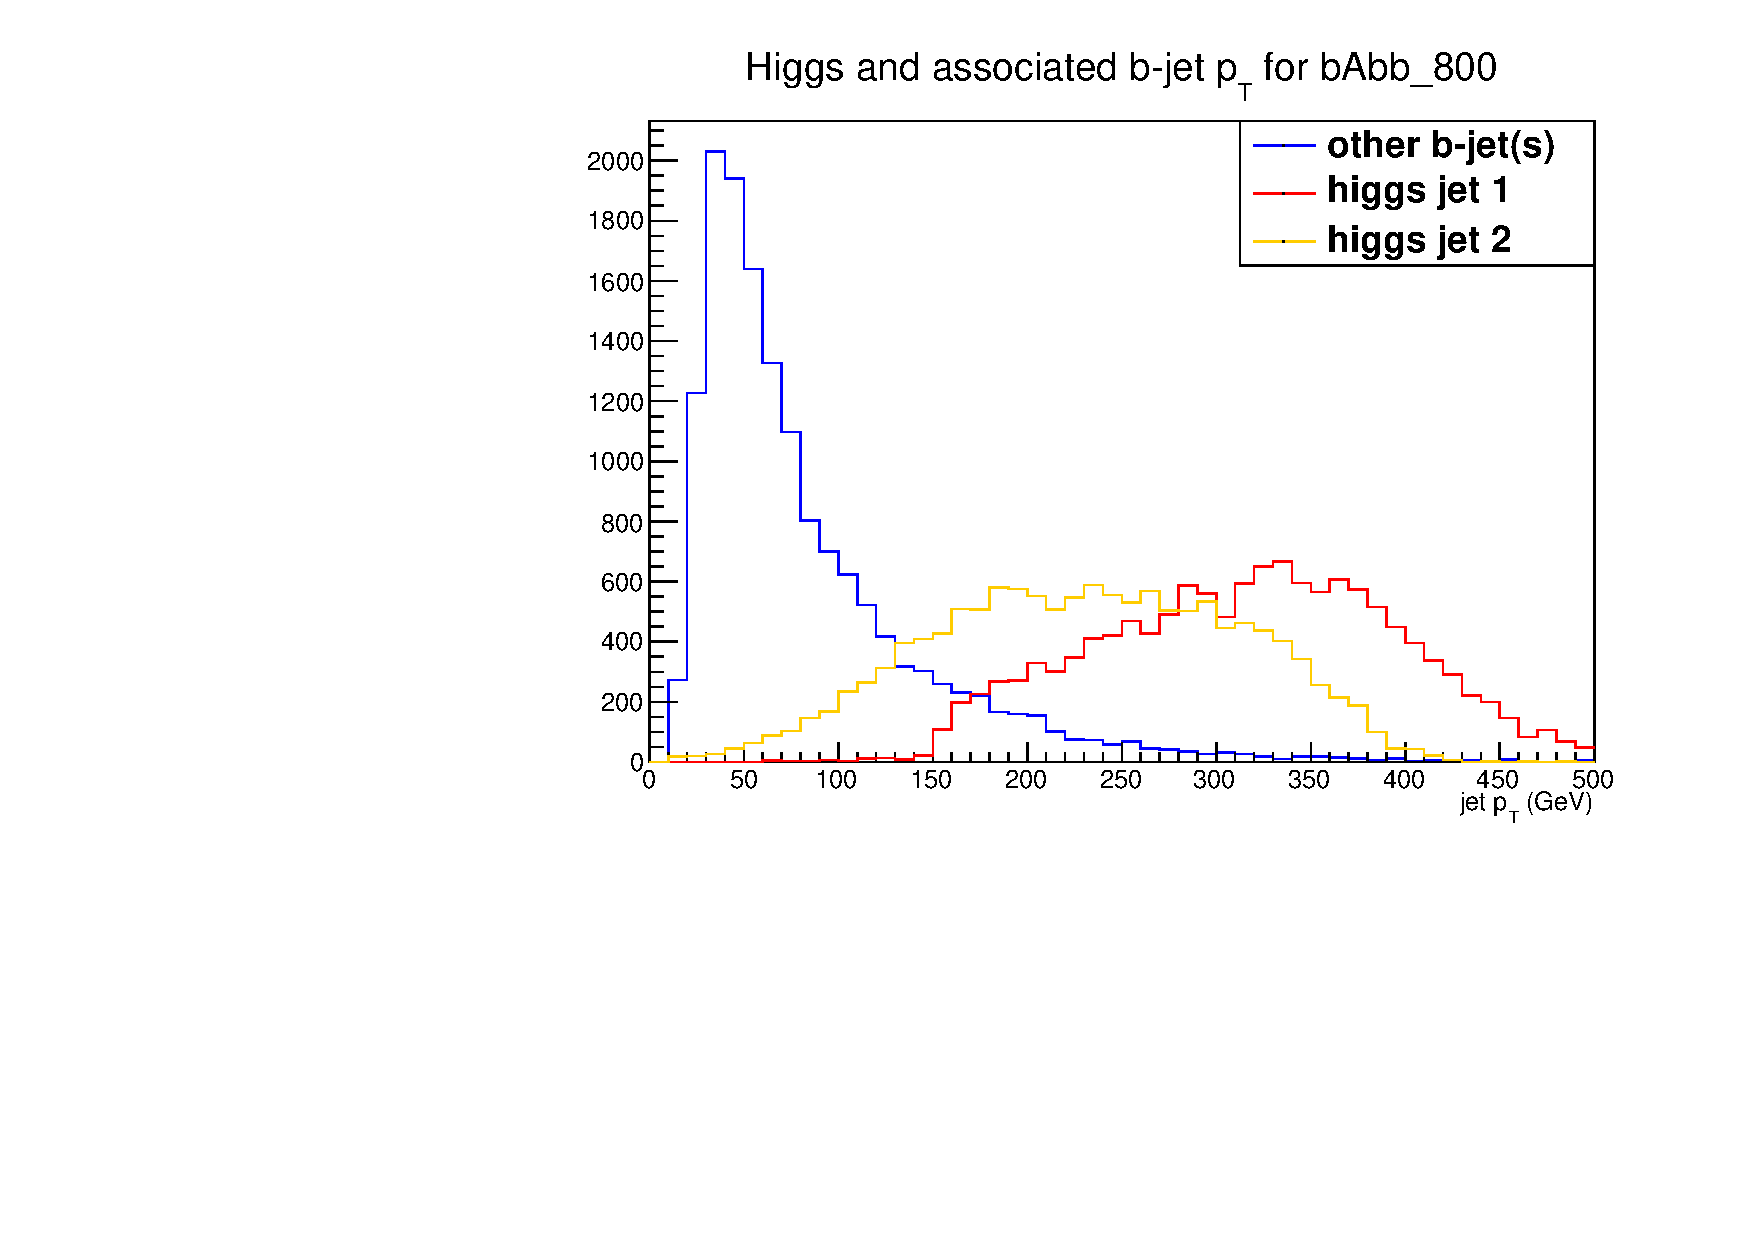
\includegraphics[width=0.3\textwidth]{SignalKin/jet_pt_compare_bAbb_800.pdf}
    \caption{The \pt of the two jets from the Higgs (classified as ``first'' and ``second'' based
    on which one has more \pt in the event), and all other $b$-tagged jet(s) in the event.
    The peaks at about 155 GeV and 55 GeV is a result of the trigger turn-on points and
    associated cut(s).  \label{fig:pt_higgs_and_associated_jets}}
\end{figure}
%----------------------------------------------

As it turns out, the presence of additional non-$b$ jets can have a significant 
effect in signal.  Since the hard scatter has only $b$-jets in the final state, the
extra jet(s) must come from other sources like initial state radiation (ISR) or 
final state radiation (FSR).  This can smear out the signal, as explained in more detail
in Section~\ref{sec:mass_res}, and combating the effects became a significant part of the
analysis.


\section{Signal Jet Combinatorics}
\label{sec:combinatorics}
An important point when trying to reconstruct the Higgs is which 2 $b$-tagged jets (of the
three available) should be used in reconstruction.  If the associated $b$-jet is accidentally
selected, then the Higgs will be mis-reconstructed and the sensitivity will suffer.  At the same time,
since the mass of the Higgs is not known, tools like a kinematic fit are not available to
help with the combinatorics.  In Figure~\ref{fig:combinatorics}, we use the MC truth
information in the signal MC to plot how often the Higgs decays to various pairs of jets
within the event; we find that especially for masses above 350 GeV or so it usually decays to
the leading and second $b$-tagged jets in the event (with about a 70\% probability).
    
\begin{figure}[hbt]
  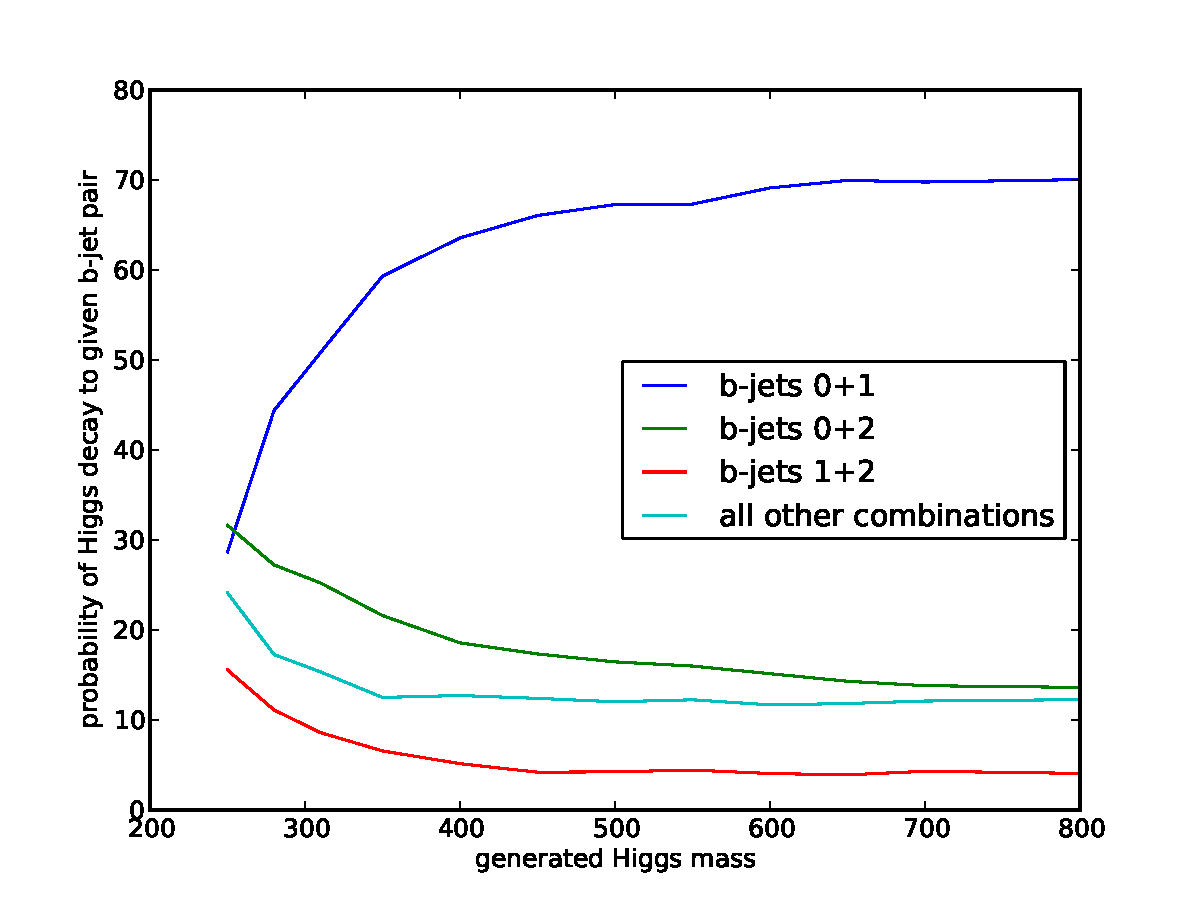
\includegraphics[width=0.78\linewidth]{SignalKin/combinatorics.pdf}
  \label{fig:combinatorics}
  \caption{The percentage probability of the Higgs decaying to a given pair of $b$-tagged jets in signal MC,
    as a function of the generated Higgs mass.  The assumption being checked is that the majority of
    the time, the Higgs decays to the leading two $b$-tagged jets (blue line), so that reconstructing with these jets
    will yield the correct combinatorics.  That assumption is correct 60-70\% of the time for $m_A>$350 GeV,
    with the remaining 30-40\% of events being spread out over many other combinations of jets.}
\end{figure}
                                                                                                                                    
                                                                                                                                    
If we require only that the leading 2 $b$-tagged jets be used in reconstruction, there can                                          
still be events in our sample where the leading 2 $b$-tagged jets in the event are not                                              
the leading 2 jets overall--for example, there can be a very hard light jet, and the $b$-tagged                                     
jets are the second and third jets in $p_T$.  When we introduce a cut that eliminates these events,                                 
by requiring that the leading 2 jets in the event be $b$-tagged, both the signal to background                                      
ratio improves (this cut is about 25\% efficient in background, and over 90\% efficient                                             
in signal) and the mass resolution is improved in signal as the events that rejected have                                           
hard FSR present and the reconstructed $m_{bb}$ is far from the generated $m_H$.    




\section{Mass Resolution}
\label{sec:mass_res}
Once the trigger and all the analysis cuts have been applied, we take the leading 2 jets in the event (which are also the leading 2 $b$-tagged jets, since we place a cut requiring that the leading 2 jets in the event be $b$-tagged) and reconstruct their combined invariant mass--if they came from a decaying particle, the reconstructed mass should be the mass of the parent particle.  On the other hand, if the leading 2 jets come from continuum QCD processes, there should be no resonance present, so we look for the presence of a resonance peak on top of a decaying power-law background.


A consistent refrain throughout this analysis is the challenge of poor mass resolution when reconstructing
the signal, especially in the low-mass tail for high values of $m_A$. The issue is important because a poorly-reconstructed (very wide)
signal peak can easily be confused with a background normalization error, which makes the analysis less
sensitive to small signals. This section will summarize the efforts to make the mass resolution as good
as possible; some tactics did produce an improvement while others did not.

\begin{itemize}
    \item REWRITE THIS LIST TO MATCH UP WITH THESIS TOPICS/ORDER
    \item require that the leading 2 jets in the event be b-tagged (improved resolution)
    \item when b-tagged jets have one or more jets nearby, include those jets in the mbb reconstruction (does
not improve resolution)
    \item when a hard ($>$80 GeV) untagged jet is present in an event, include it in the mbb reconstruction
(does not improve resolution)
\end{itemize}
However, the mass resolution remains an issue. The problem is significantly worse at higher masses;
to some extent, this is inevitable because the inherent width of the Higgs resonance increases with mA
(quantification of this ect can be found in Table 5. However, the inherent width goes up to about 12
GeV (at mA=800 GeV), while the width of the reconstructed mass peak goes up to several hundred GeV.
With this in mind, it’s clear that other ects drive the mass resolution. Thishe sensitivity of this analysis depends on the signal cross section and efficiency, the background cross section and efficiency, but also the signal resolution.  The broader the signal mass peak, the more difficult it is to distinguish from the background.  

Unfortunately, the mass resolution significantly degrades as a $m_A$ grows.  Some of this is due to the inherent width growing as $m_A$ grows, as can be seen in Table~\ref{tab:sig_mc_parameters}.  

\subsection{Mass Resolution Improvement after Requiring that Leading Two Jets be $b$-Tagged}
The mass resolution also improves when we require that the leading two jets in the event be b-tagged;
 the plots in Figure 39 and Figure 40 show the ect on the invariant mass distribution.
 In order to quantify the mass resolution ect, we define the “left” and “right” shoulders of the mbb
 distribution, which are respectively the portion of the mbb distribution that are below and above the peak.
 go into further detail on the signal shape in Section 6.2; but in Table~\ref{tab:signal_mass_RMS_compare} the RMS of especially the left
 shoulder before and after requiring b-tags on the leading 2 jets quantitatively shows the mass resolution
 improvement.



%----------------------------------------------
\begin{table}
\centering
\caption{The RMS of the mass distribution in the left and right shoulders of the peak,
    as explained in the text.  The left shoulder is dominated by radiation off the Higgs
    and/or the Higgs daughter jets in addition to combinatorial mis-reconstructions,
    leading to a larger RMS than the right shoulder, which
    is dominated by combinatorics only.\label{tab:signal_mass_RMS_compare}   }
  \begin{tabular}{ccccc}
     \hline \hline
     mass (GeV) & \multicolumn{2}{c}{$b$-tags on leading jets (GeV)} & \multicolumn{2}{c}{no $b$-tags on leading jets (GeV)}  \\
        & left & right & left & right \\ \hline
     250 & 13.5 & 89.2 & 36.7 & 87.7 \\
     280 & 19.2 & 68.8 & 27.5 & 71.4 \\
     310 & 19.2 & 58.3 & 31.8 & 58.1 \\
     350 & 28.3 & 34.5 & 33.9 & 36.2 \\
     400 & 33.4 & 26.1 & 45.1 & 26.5 \\
     450 & 39.5 & 25.7 & 62.2 & 25.9 \\
     500 & 48.6 & 29.3 & 81.1 & 29.8 \\
     550 & 54.9 & 31.1 & 93.1 & 33.3 \\
     600 & 73.0 & 26.0 & 117.6 & 30.5 \\
     650 & 75.4 & 31.7 & 130.8 & 31.8 \\
     700 & 75.7 & 40.3 & 143.4 & 40.7 \\
     800 & 100.9 & 36.2 & 177.4 & 36.3 \\
     \hline     \end{tabular}
\end{table}
%----------------------------------------------






\subsection{Validation of Qualitative Shape Differences}
The first question to ask is whether the high-mass mbb distributions are qualitatively lower-resolution than
the low-mass distributions–in other words, whether the ratio of the width to the generated mass changes
as a function of mass. We probe this by “normalizing” the signal MC mass, dividing each entry in the mbb
histogram by the nominal mass which was generated; for example, a signal MC event that was generated
with a Higgs mass of 350 GeV and reconstructed to have 300 GeV would be entered into the histogram
as (300/350). Repeating this normalization process for several mass points allows us to compare the
shapes for different $m_A$ values.
We find that even when the mbb distributions are renormalized, the high-mass distributions remain
wider than the low-mass distributions. That points toward FSR as a likely culprit, and in the following
sections we will detail several attempts at FSR recovery.
\begin{figure}[hbt]
  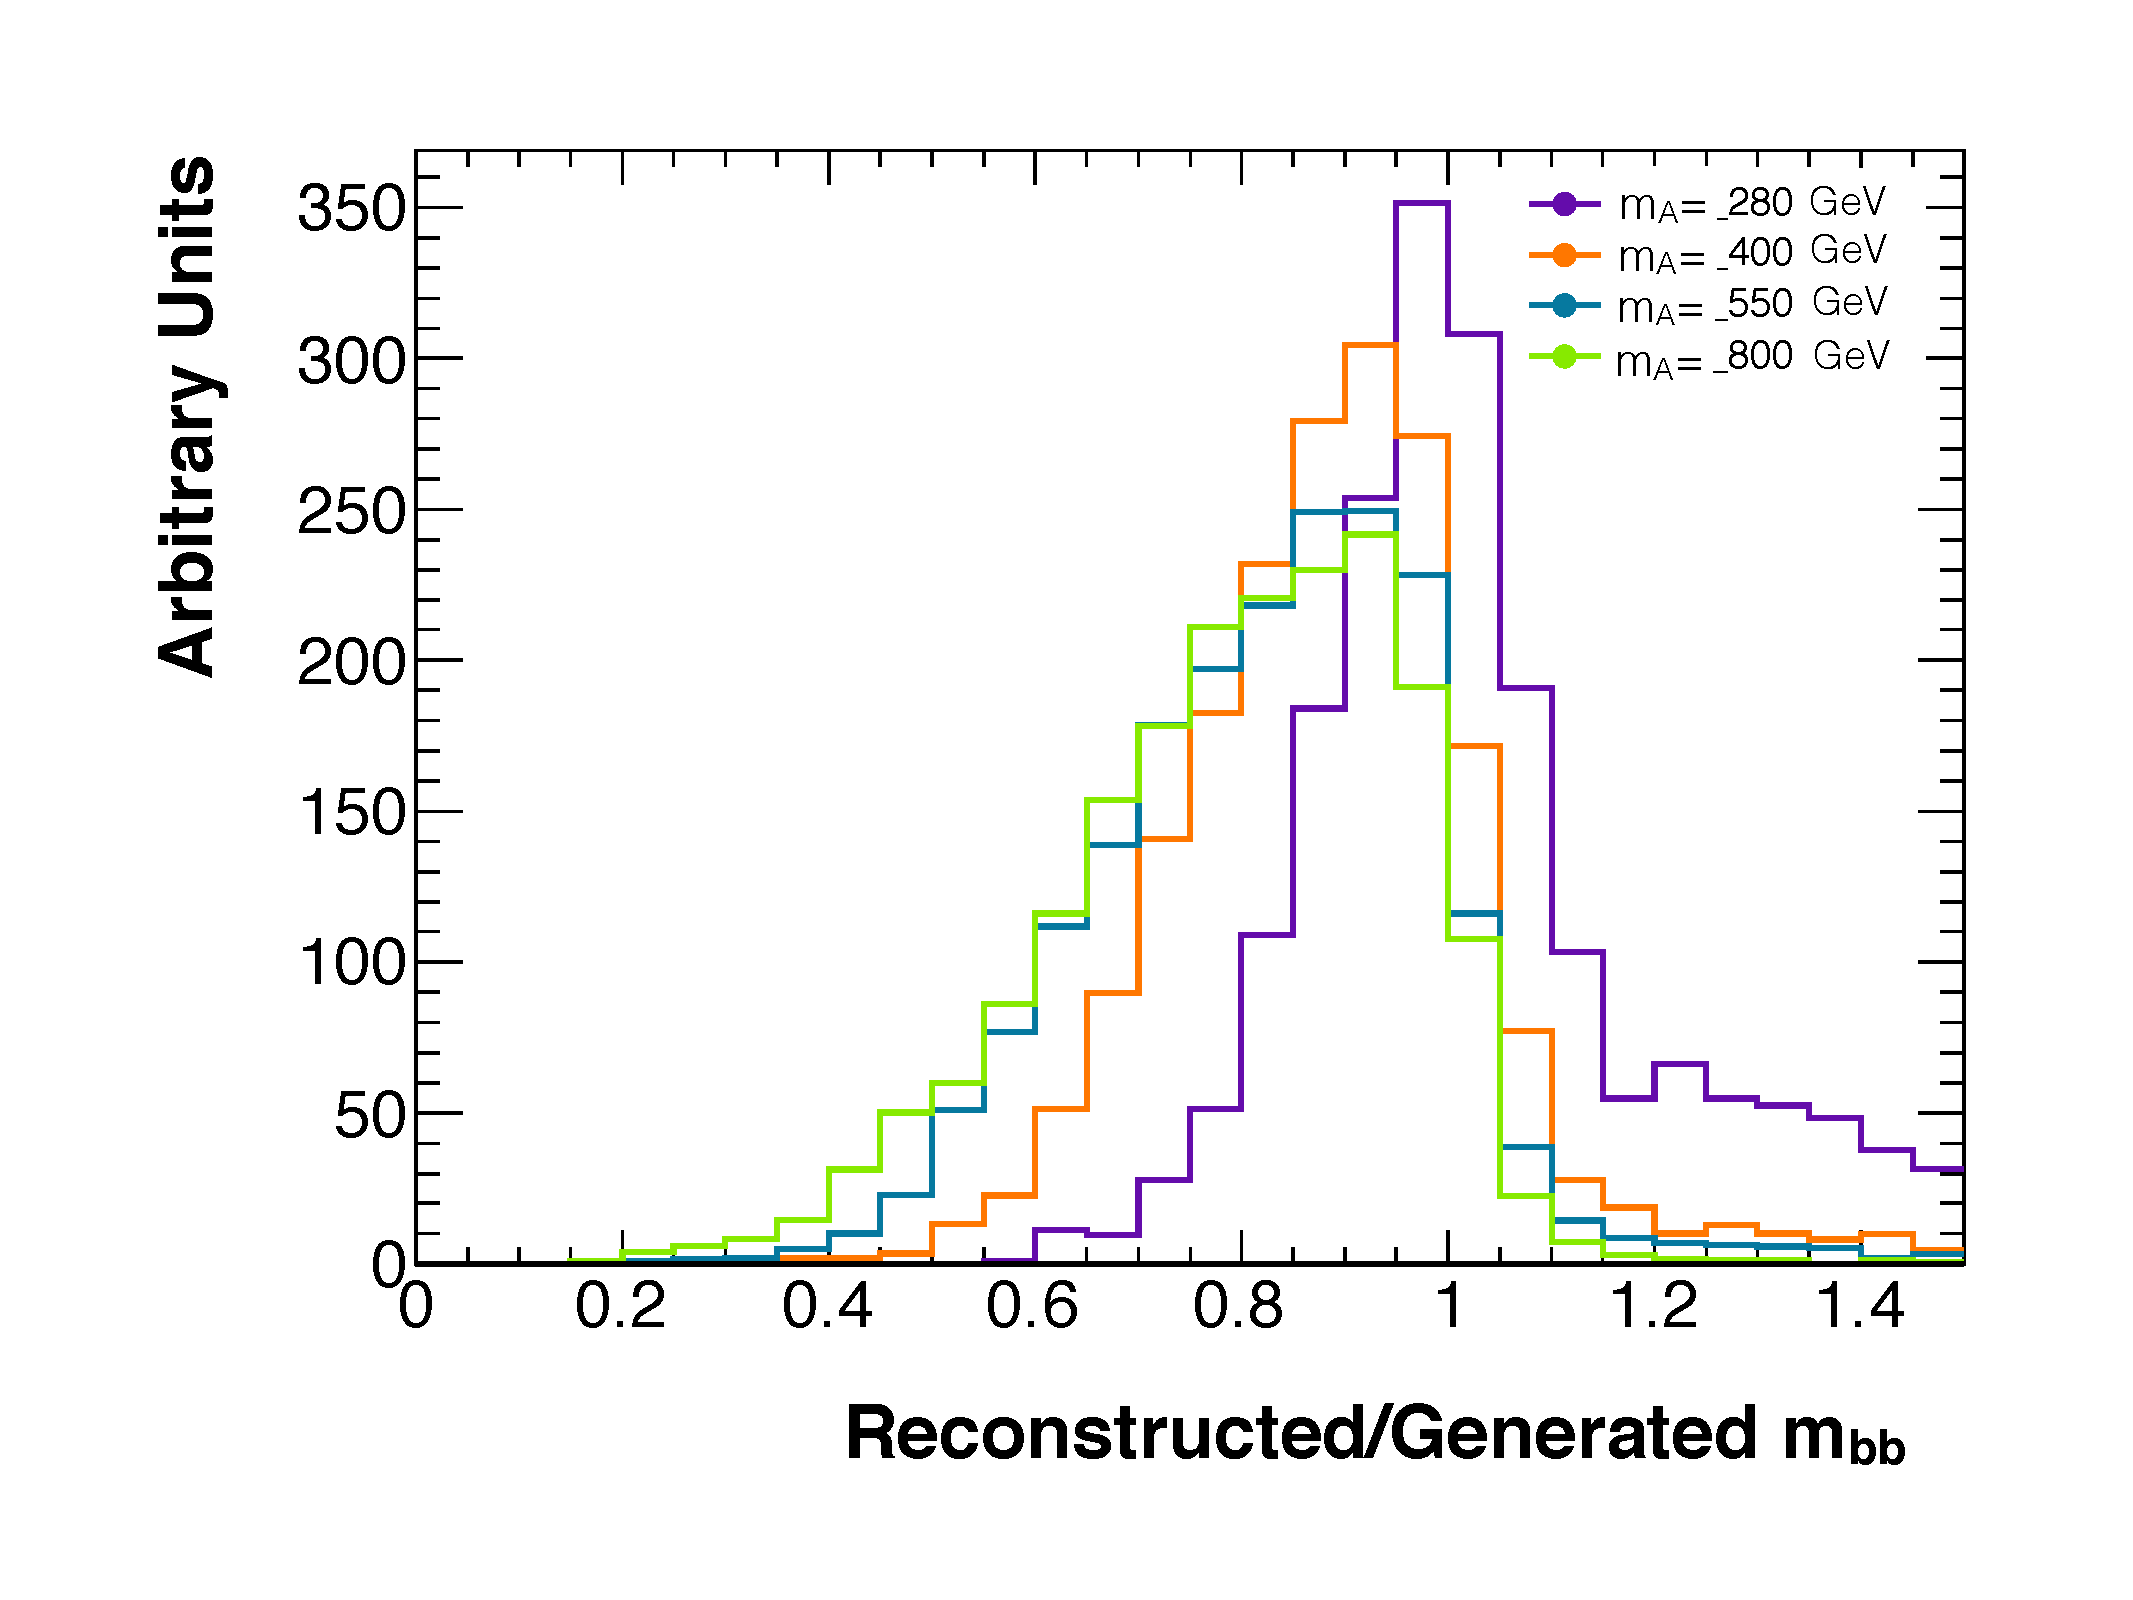
\includegraphics[width=0.78\linewidth]{SignalKin/mbb_normalized_signal.pdf}
  \label{fig:mbb_norm}
  \caption{The normalized $m_{bb}$ distributions for several signal mass points}
\end{figure}





\subsection{Jet Modifications}
\subsection{Topology-Based Energy Recovery Algorithm}
 One hypothesis for the distribution of the FSR is that, for the high-\pt jets that result from the Higgs
 daughter b-quarks, they might radiate away partons that are hard enough to be clustered into their own
 jets (\pt$>$25 GeV) but end up nearby the leading jets in the detector (where nearby is defined as within
 dR$<$1.0). In other words, we look for a topology where there are one or more jets near one of the leading
2 jets, and in cases where such jets are found, we add them back in when reconstructing mbb.
 This is found to have little ect on the mass resolution. In practice, only about 20\% of events
 have the topology where additional jet(s) are found near the leading 2 jets, and the mass resolution
 looks virtually unchanged before and after adding this correction. This suggests a couple of possible
 conditions: either the FSR is too diffuse and/or low-energy to be clustered into jets, and/or it is farther
 than the dR $<$ 1.0 search zone allows for recovery. 
    
\begin{figure}[hbt]
  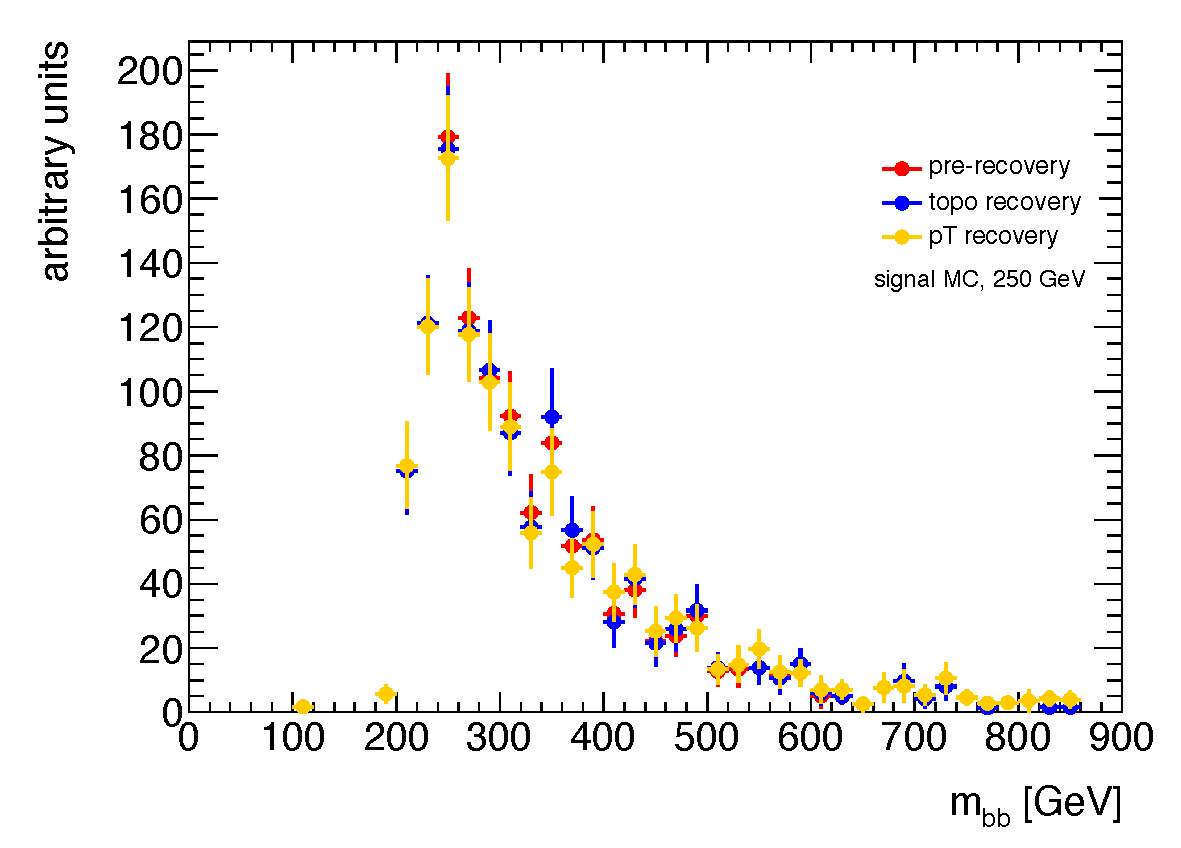
\includegraphics[width=0.45\linewidth]{SignalKin/fsr_recovery_bAbb_250.pdf}
  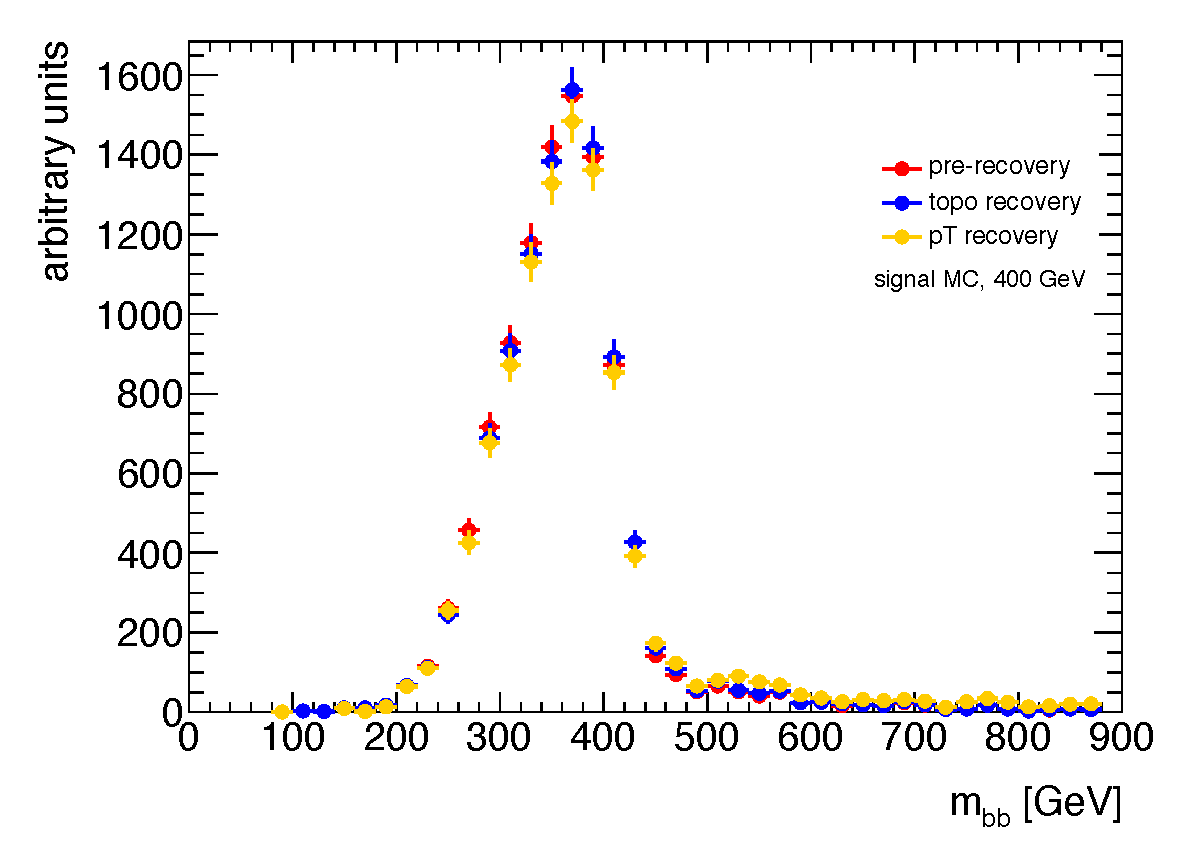
\includegraphics[width=0.45\linewidth]{SignalKin/fsr_recovery_bAbb_400.pdf}
\newline
  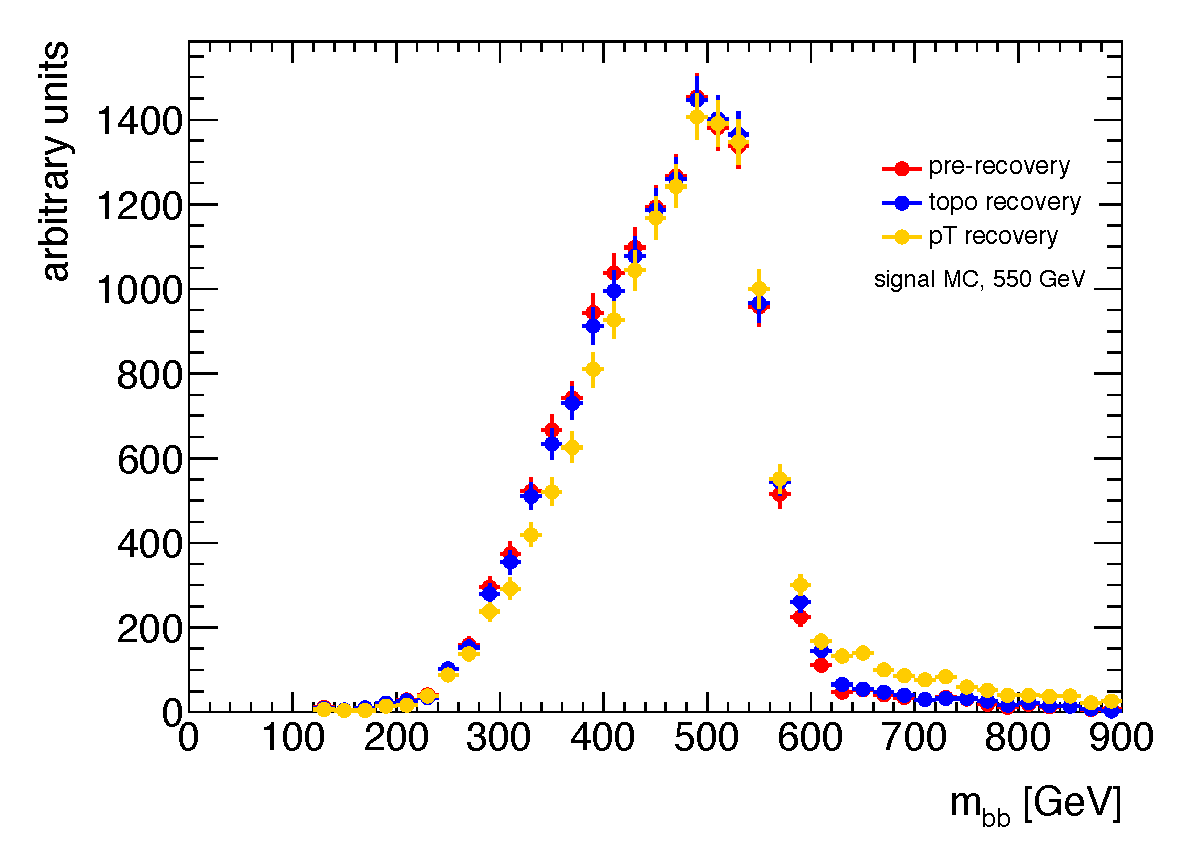
\includegraphics[width=0.45\linewidth]{SignalKin/fsr_recovery_bAbb_550.pdf}
  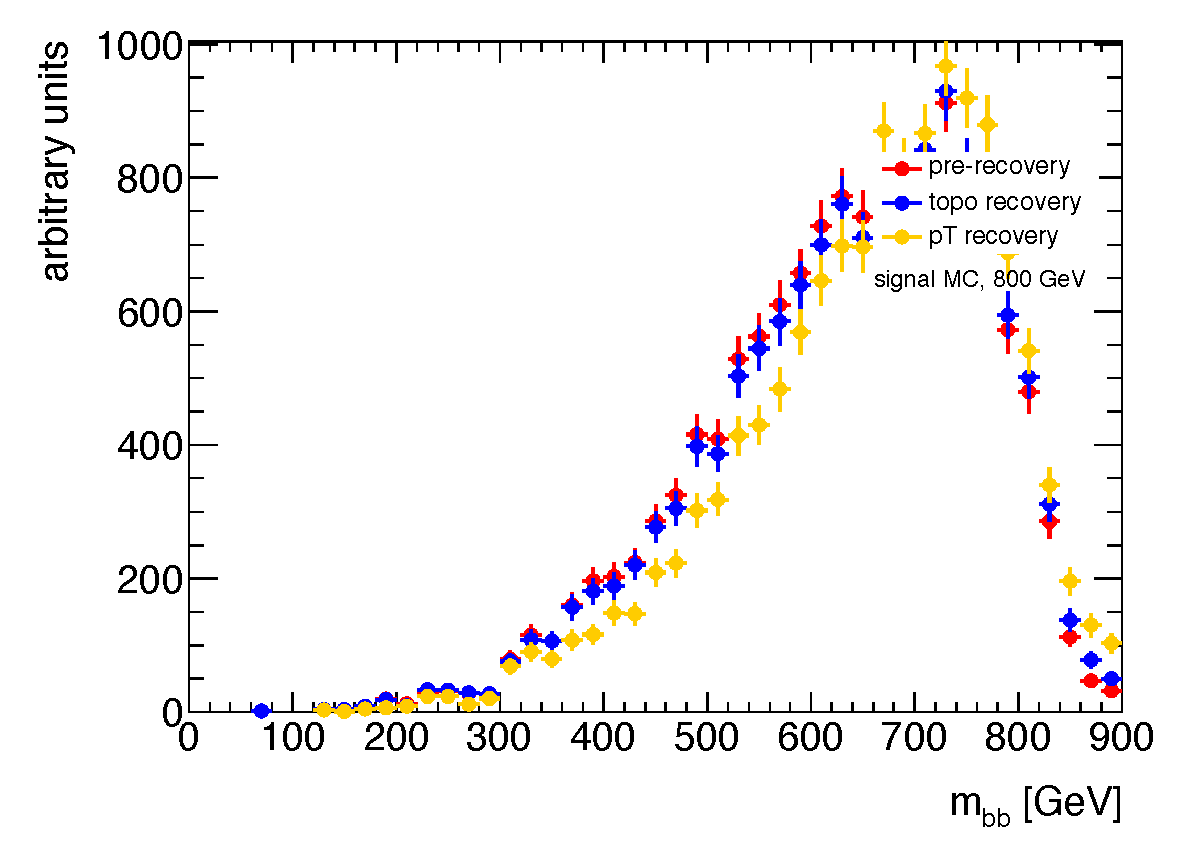
\includegraphics[width=0.45\linewidth]{SignalKin/fsr_recovery_bAbb_800.pdf}
  \label{fig:fsr_recovery}
  \caption{The $m_{bb}$ distributions out-of-the-box, and after attempting the $p_T$-based and topology-based FSR recovery algorithms, for several signal mass points.}
\end{figure}



\subsection{\pt-Based Energy Recovery Algorithm}
The \pt-based energy recovery algorithm is based on the idea that perhaps the FSR takes the form of one
 or two very high-energy radiated particles that can end up far away from the leading 2 jets but can be
 identified by their high pT . In practice, what this means is looking for events with a non-b-tagged jet that
 has \pt$>$80 GeV, and when one is found, adding this back in when reconstructing mbb.
 Unfortunately the ect on the mass resolution is negligible. A few events move out of the low-mass
 tail, and the high-mass tail gets a few more events as jets can be mistakenly added back in even when no
 FSR was lost.

\subsection{$n_{jets}$ Dependence} 
\begin{figure}[hbt]
  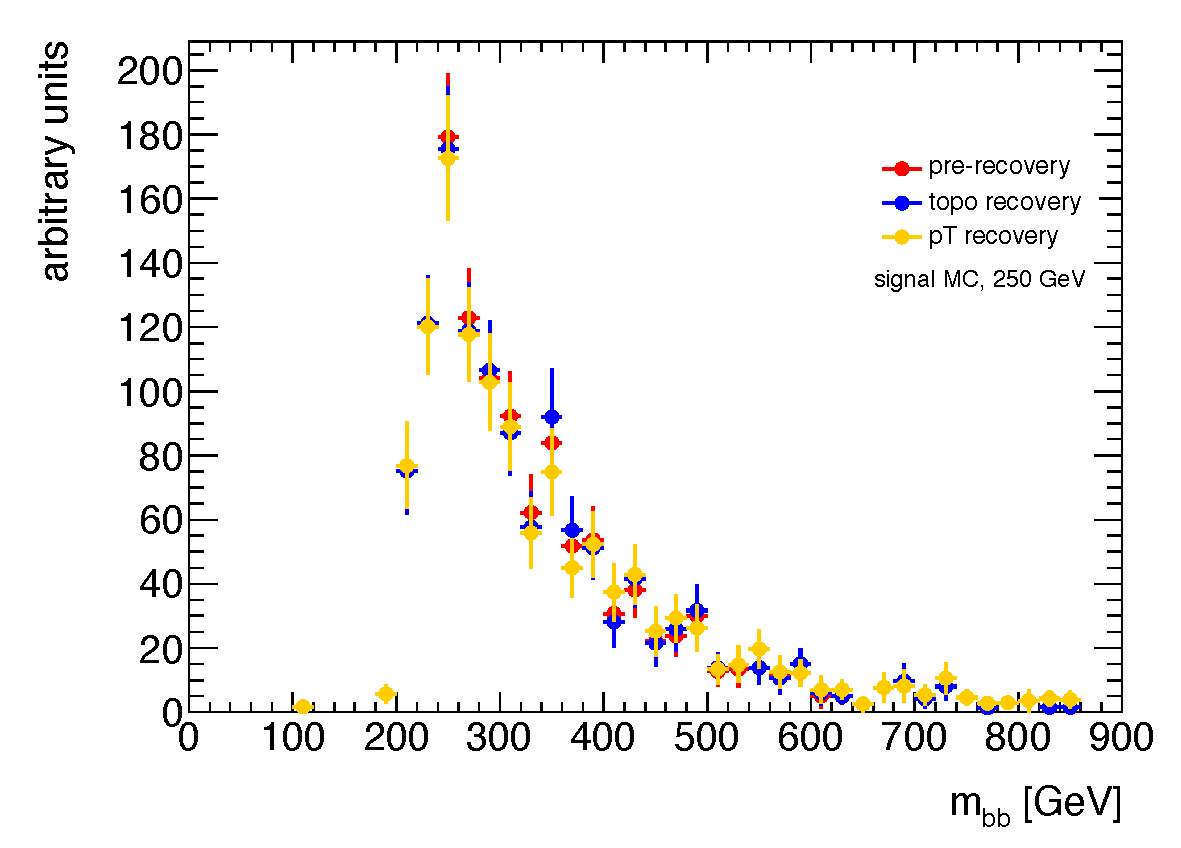
\includegraphics[width=0.45\linewidth]{SignalKin/fsr_recovery_bAbb_250.pdf}
  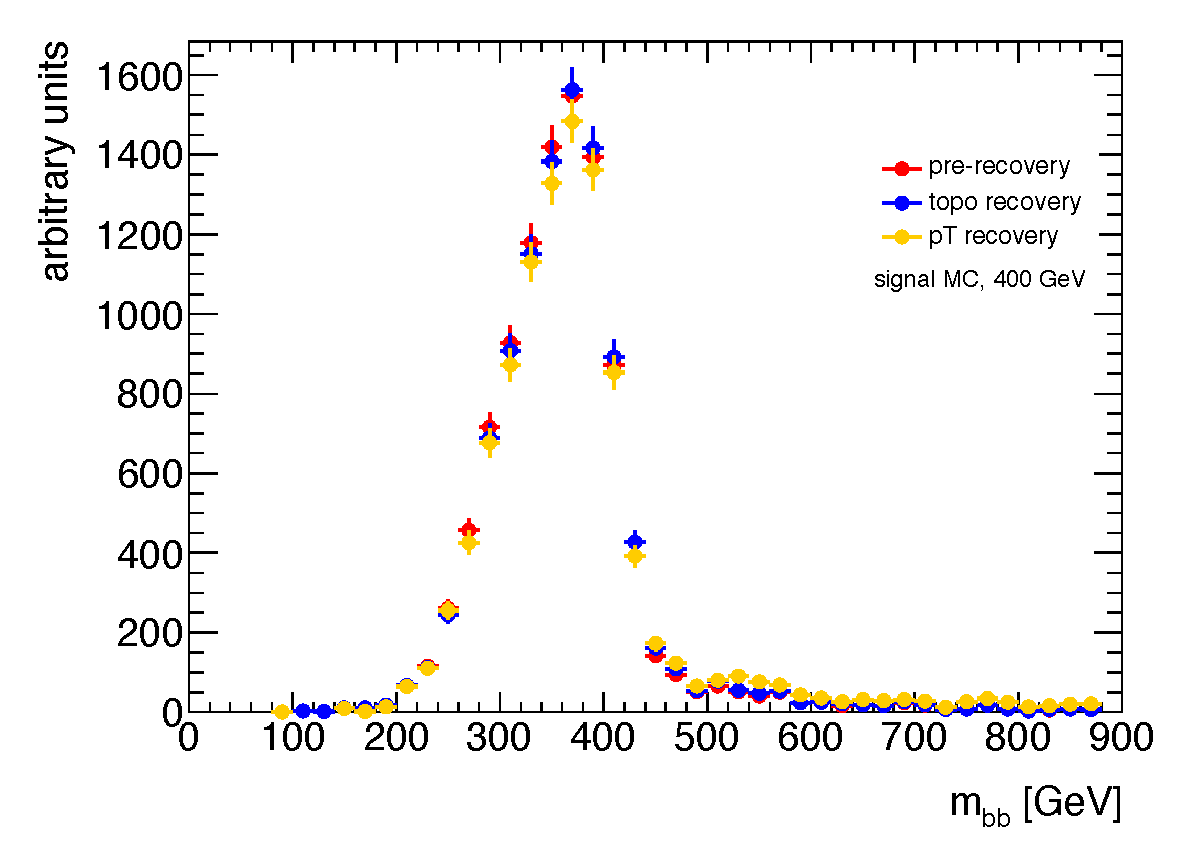
\includegraphics[width=0.45\linewidth]{SignalKin/fsr_recovery_bAbb_400.pdf}
\newline
  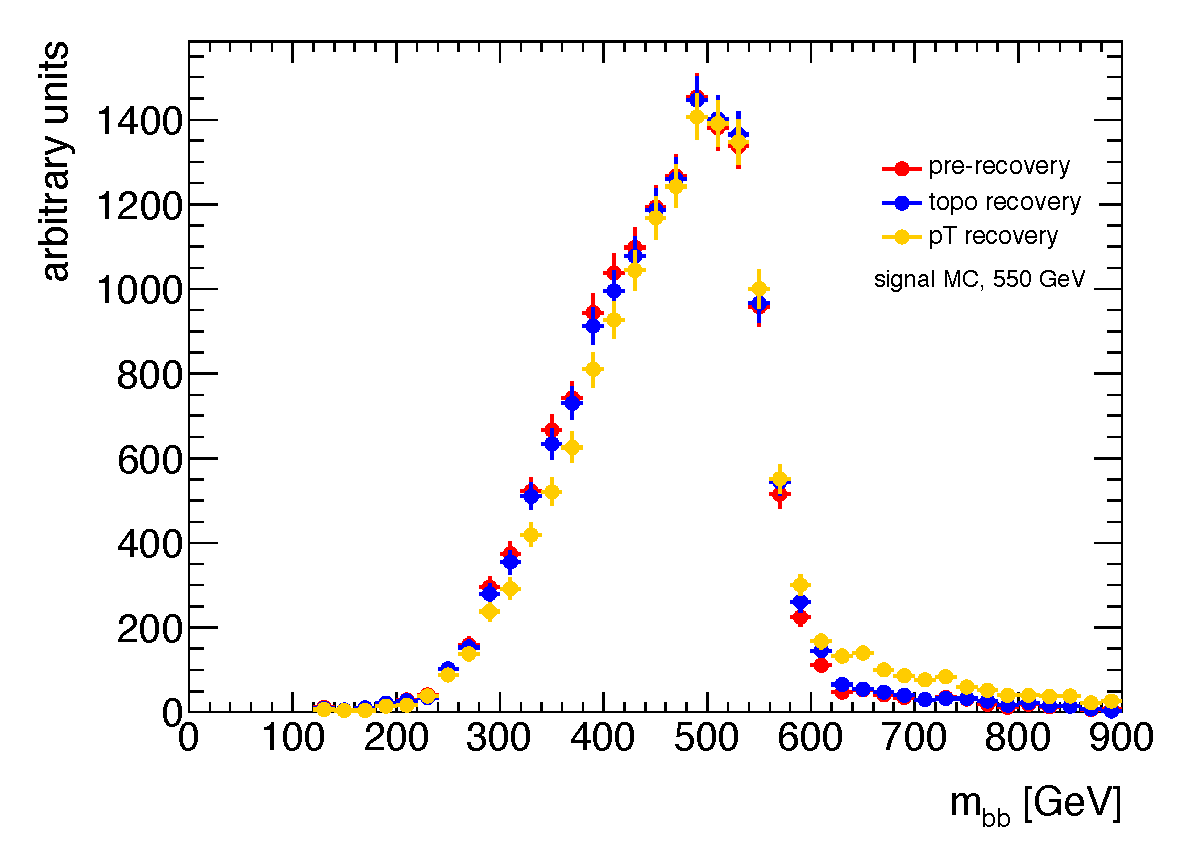
\includegraphics[width=0.45\linewidth]{SignalKin/fsr_recovery_bAbb_550.pdf}
  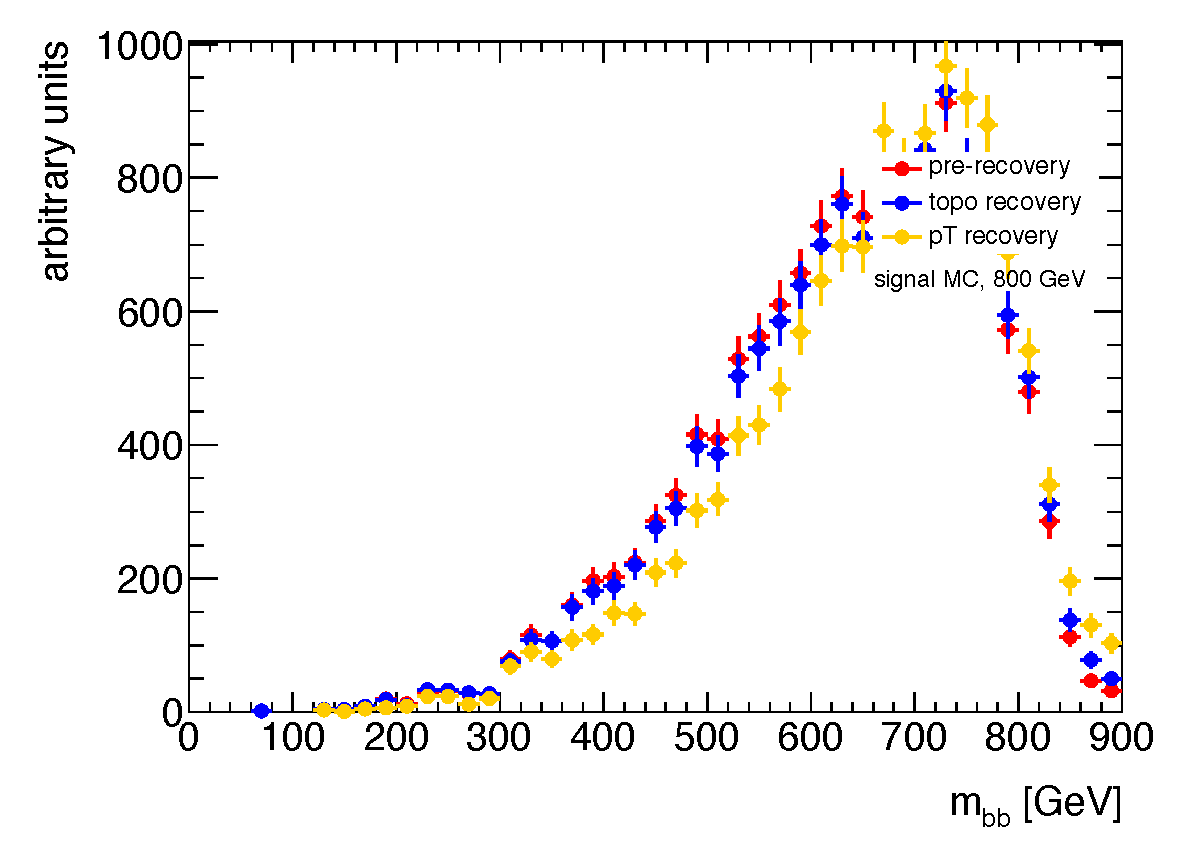
\includegraphics[width=0.45\linewidth]{SignalKin/fsr_recovery_bAbb_800.pdf}
  \label{fig:mbb_njets_signal}
  \caption{The $m_{bb}$ distributions at a few representative mass points in signal MC, as a function of the number of jets in the event.  
    The 5+ jets bin contains all events with 5 jets or more.}
\end{figure}
